%&header

\documentclass[a4paper,DIV=15]{scrartcl}


\usepackage{amsmath}
\usepackage{subcaption}
%
\usepackage{graphicx}
\usepackage{tabularx}
\usepackage{makecell}
\usepackage{booktabs}
\usepackage{rotating}
\usepackage{float}
\usepackage{layouts}
\usepackage{pgf}
\usepackage{fancyvrb}

\usepackage{todonotes}
\usepackage[hidelinks]{hyperref}

\usepackage{tikz}

\usepackage{crimson}
\usepackage{newtxmath}
\usepackage{polyglossia}
\usepackage[natbib=true,style=authoryear,backend=biber]{biblatex}
\usepackage{microtype}
\usepackage{minted}
\usepackage{xstring}
\usepackage{newunicodechar}

\usepackage[column=C]{cellspace}

\usepackage[bottom=2.5cm,top=2.0cm,left=2.4cm,right=2.4cm]{geometry}

\usepackage[detect-all,binary-units,separate-uncertainty=true,round-mode=uncertainty,input-digits={0123456789ABCDEF}]{siunitx}

\setdefaultlanguage{english}

\NewCommandCopy{\oldautocite}{\autocite}
\renewcommand{\autocite}[1]{ \oldautocite{#1}}

\cellspacetoplimit4pt
\cellspacebottomlimit4pt



\usepackage[toc]{glossaries}

\renewcommand\cellalign{lc}

\ExecuteBibliographyOptions{mincrossrefs=100}

\makeglossaries

% \usepackage{nomencl}
% \let\abbrev\nomenclature
% \renewcommand{\nomname}{List of Abbreviations}
% \setlength{\nomlabelwidth}{.25\hsize}
% \renewcommand{\nomlabel}[1]{#1 \dotfill}
% \setlength{\nomitemsep}{-\parsep}
% %\makeglossary
% \makenomenclature%
% \newcommand{\markup}[1]{\uline{#1}}
% \usepackage{makeidx}                              % index of key words
% \makeindex

\raggedbottom%


\newcommand{\thesisTitle}{Implementation of an \FPGA{}-based memory mapped buffer for real-time communication with a neuromorphic \ASIC{}}
\newcommand{\thesisTitleGerman}{Entwicklung eines \FPGA{}-basierten memory-mapped Zwischenspeicher für Echtzeit-Kommunikation mit einem neuromorphen \ASIC{}}

\providecommand*{\listingautorefname}{Listing}



\usetikzlibrary{external}
\tikzexternalize[up to date check={simple},prefix=./external_figures/]
\usetikzlibrary{arrows,arrows.meta,bending,positioning,calc,patterns,backgrounds,fit,decorations.pathreplacing,shapes.geometric}

\newcommand\MeanStdValue[2]{%
  \ensuremath{%
    \SI{\csname #1Mean\endcsname \pm \csname #1Std\endcsname}{#2}%
  }%
}

% ugh
\newcommand{\inputtikz}[1]{\StrSubstitute{#1}{/}{-}[\filename]\StrSubstitute{\filename}{.}{-}[\filenameNew]\tikzsetnextfilename{\filenameNew}\input{#1}}

\newcommand{\inputpgf}[1]{
\StrSubstitute{#1}{/}{-}[\filename]\StrSubstitute{\filename}{.}{-}[\filenameNew]\tikzsetnextfilename{\filenameNew}%
\begin{tikzpicture}\node[inner sep=0pt]{\input{#1}};\end{tikzpicture}%
}%

\definecolor{color0}{HTML}{1f77b4}  % blue
\definecolor{color1}{HTML}{ff7f0e}  % orange
\definecolor{color2}{HTML}{2ca02c}  % green
\definecolor{color3}{HTML}{d62728}  % red
\definecolor{color4}{HTML}{9467bd}  % purple
\definecolor{color5}{HTML}{8c564b}  % red-gray
\definecolor{color6}{HTML}{e377c2}  % pink
\definecolor{color7}{HTML}{7f7f7f}  % gray
\definecolor{color8}{HTML}{bcbd22}  % incredibly ugly yellow-gray
\definecolor{color9}{HTML}{17becf}  % light blue

% colors for multi-compartment illustrations
\colorlet{comp0}{color1!60}
\colorlet{comp1}{color5!60}
\colorlet{comp2}{color8!60}
\colorlet{comp3}{color2!60}
\colorlet{comp4}{color3!60}
\colorlet{comp5}{color6!60}

% \tikzset{external/system call={lualatex -halt-on-error -shell-escape -interaction=batchmode -fmt header -jobname "\image" "\texsource"}}

% ugh
\makeatletter
\renewcommand{\todo}[2][]{\tikzexternaldisable\@todo[#1]{#2}\tikzexternalenable}
\makeatother

\newunicodechar{α}{\alpha}
\newunicodechar{Α}{\alpha}
\newunicodechar{β}{\beta}
\newunicodechar{Β}{\beta}
\newunicodechar{γ}{\gamma}
\newunicodechar{δ}{\delta}
\newunicodechar{ε}{\varepsilon}
\newunicodechar{Ε}{\varepsilon}
\newunicodechar{ζ}{\zeta}
\newunicodechar{η}{\eta}
\newunicodechar{θ}{\theta}
\newunicodechar{ι}{\iota}
\newunicodechar{κ}{\kappa}
\newunicodechar{λ}{\lambda}
\newunicodechar{μ}{\mu}
\newunicodechar{Μ}{\Mu}
\newunicodechar{ν}{\nu}
\newunicodechar{ξ}{\xi}
\newunicodechar{ο}{\omicron}
\newunicodechar{π}{\pi}
\newunicodechar{Π}{\Pi}
\newunicodechar{ρ}{\rho}
\newunicodechar{Ρ}{\Rho}
\newunicodechar{σ}{\sigma}
\newunicodechar{τ}{\tau}
\newunicodechar{Τ}{\Tau}
\newunicodechar{υ}{\upsilon}
\newunicodechar{φ}{\varphi}
\newunicodechar{χ}{\chi}
\newunicodechar{ψ}{\psi}
\newunicodechar{ω}{\omega}
\newunicodechar{∀}{\forall}
\newunicodechar{×}{\times}
\newunicodechar{Γ}{\Gamma}
\newunicodechar{Δ}{\Delta}
\newunicodechar{∃}{\exists}
\newunicodechar{ℤ}{\mathbb{Z}}
\newunicodechar{∧}{\wedge}
\newunicodechar{Θ}{\Theta}
\newunicodechar{⇒}{\implies}
\newunicodechar{∩}{\cap}
\newunicodechar{Λ}{\Lambda}
\newunicodechar{∫}{\int}
\newunicodechar{ℕ}{\mathbb{N}}
\newunicodechar{Ξ}{\Xi}
\newunicodechar{∇}{\nabla}
\newunicodechar{Π}{\Pi}
\newunicodechar{ℝ}{\mathbb{R}}
\newunicodechar{Σ}{\Sigma}
\newunicodechar{⇔}{\iff}
\newunicodechar{Υ}{\Upsilon}
\newunicodechar{Φ}{\Phi}
\newunicodechar{ℂ}{\mathbb{C}}
\newunicodechar{Ψ}{\Psi}
\newunicodechar{Ω}{\Omega}
\newunicodechar{ϑ}{\vartheta}
\newunicodechar{∞}{\infty}
\newunicodechar{∈}{\in}
\newunicodechar{⊂}{\subset}
\newunicodechar{ϰ}{\varkappa}
\newunicodechar{ϕ}{\phi}
\newunicodechar{∨}{\vee}
\newunicodechar{∮}{\oint}
\newunicodechar{↦}{\mapsto}
\newunicodechar{ℚ}{\mathbb{Q}}
\newunicodechar{⊆}{\subseteq}
\newunicodechar{⊊}{\subsetneq}
\newunicodechar{∪}{\cup}
\newunicodechar{·}{\cdot}


\addbibresource{bib.bib}
\addbibresource{vision.bib}

% \pagestyle{scrheadings}

% \usemintedstyle{tango}
\usemintedstyle{friendly}
\setminted[]{breaklines=true,linenos,frame=lines,mathescape=true,tabsize=4}

% \title{ba writeup}
% \author{Robin Heinemann}
% \date{February 2023}

\newcommand\code[1]{\detokenize{#1}}

\newcommand\HWinTheLoop{hardware in-the-loop}

\newcommand\emitDummyInstr{\texttt{\Verb|emit_dummy(N)|}}
\newcommand\haltInstr{\texttt{\Verb|halt()|}}
\newcommand\resetSleepInstr{\texttt{\Verb|reset_sleep()|}}

\newcommand\systime{systime}
\newcommand\traceArb{trace arbitration}

\newcommand\allocator{allocator}

\newcommand\linear{linear}
\newcommand\random{random}
\newcommand\randomDense{random dense}
\newcommand\interleaved{interleaved}
\newcommand\interleavedDense{interleaved dense}

\newcommand\rtt{round trip time}

\newcommand\testnode{\texttt{EpycHost1}}

\newcommand\xcelium{xcelium}
\newcommand\xceliumVer{21.03-s009}


\newcommand\DPI{DPI}
\newcommand\PhyWordSize{\SI{64}{\bit}}
\newcommand\JTAG{JTAG}
\newcommand\JTAGID{JTAGID}
\newcommand\taildesc{taildesc}
\newcommand\curdesc{curdesc}
\newcommand\RCF{RCF}
\newcommand\uvmframework{UVM}
\newcommand\completed{completed}
\newcommand\Xilinx{Xilinx}
\newcommand\pbexec{pbexec}
\newcommand\ASIC{ASIC}
\newcommand\ayo{ayo}
\newcommand\vfifo{vfifo}
\newcommand\smartconnect{smartconnect}
\newcommand\LVDS{LVDS}

\newcommand\DDR{DDR3}
\newcommand\MMToS{MM2S}
\newcommand\SToMM{S2MM}

\newcommand\descriptor{descriptor}
\newcommand\HostARQ{Host-ARQ}
\newcommand\systemverilog{SystemVerilog}

\newcommand\waitCat{wait category}

\newcommand\DRAM{DRAM}

\newcommand\MIG{MIG}

\newcommand\AW{AW}
\newcommand\NEXT{NEXT}
\newcommand\LAST{LAST}
\newcommand\TVALID{TVALID}
\newcommand\AR{AR}
\newcommand\ACLK{ACLK}
\newcommand\AXILite{AXI-Lite}
\newcommand\ARESETn{ARESETn}
\newcommand\READY{READY}
\newcommand\TLAST{TLAST}
\newcommand\VALID{VALID}

\newcommand\XilinxMIG{XilinxMIG}
\newcommand\API{API}
\newcommand\IPv{IPv}
\newcommand\readCat{read category}

\newcommand\BSSTwo{BSS2}
\newcommand\bssTwoOS{\BSSTwo{} OS}

\newcommand\halfduplex{half-duplex}

\newcommand\pbExecClock{\ensuremath{\SI{125}{\mega\hertz}}}

\newcommand\Gigabitethernet{Gigabit Ethernet}

\newcommand\pbExecBandwidth{\ensuremath{\SI{8}{\giga\bit\per\second}}}

\newcommand\python{Python}
\newcommand\Kintex{Kintex}
\newcommand\UTEncoder{UTEncoder}
\newcommand\vpi{VPI}
\newcommand\cocotb{cocotb}
\newcommand\dpi{dpi}
\newcommand\DMA{DMA}
\newcommand\pbmem{pbmem}
\newcommand\FPGA{FPGA}
\newcommand\construct{construct}
\newcommand\ASICBandwidth{\ensuremath{\SI{8}{\giga\bit\per\second}}}
\newcommand\writeCat{write category}
\newcommand\SIMMEMSIZE{\ensuremath{\SI{32}{\mebi\byte}}}
\newcommand\cocotbaxi{cocotbaxi}

\newcommand\AXI{AXI}
\newcommand\FIFO{FIFO}

\newcommand\bramctrl{bramctrl}

\newcommand\vhpi{VHPI}

\newcommand\TKEEP{TKEEP}
\newcommand\TDATA{TDATA}

\newcommand\globalfence{globalfence}

\newcommand\AXIDMA{AXIDMA}
\newcommand\Ethernet{Ethernet}

\newcommand\hdl{HDL}
\newcommand\UDP{UDP}

\newcommand\R{R}
\newcommand\AXIBRAMController{AXIBRAMController}


\newcommand\PlaybackProgram{playback program}

\newcommand\TREADY{TREADY}

\newcommand\cpp{cpp}

\newcommand\UT{UT}

\newcommand\burstsize{burst size}

\newcommand\VPI{VPI}

\newcommand\flangedram{flange-dram}

\newcommand\RAM{RAM}

\newcommand\ValidNextStream{ValidNext stream}

\newcommand\AXIRAM{AXIRAM}
\newcommand\flange{flange}

\newcommand\mmap{mmap}

\newcommand\VFIFO{VFIFO}
\newcommand\FAXI{FAXI}

\newcommand\HostBandwidth{\SI{1}{\giga\bit\per\second}}

\newcommand\hxcomm{hxcomm}

\newcommand\B{B}
\newcommand\W{W}
\newcommand\AXIStream{AXI-Stream}

\newcommand\wait{wait}

\newcommand\DUT{DUT}

\input{data/bandwidth}


% \renewcommand\autocite[1]{??}

\begin{document}

\pagestyle{empty}
\begin{titlepage}
\begin{center}
 
\Large\textbf{Department of Physics and Astronomy\\
Heidelberg University}

\vspace{18cm}

\normalsize
Bachelor Thesis in Physics\\
submitted by\\
\vspace{0.5cm}
\Large\textbf{Robin Heinemann}\\
\normalsize
\vspace{0.5cm}
born in Kassel (Germany)\\
\vspace{0.5cm}
\Large\textbf{2023}
\normalsize

\newpage




\Large\textbf{Implementation of a memory mapped playback and trace buffer for communication with neuromorphic ASICs}

\vspace{18cm}

\normalsize
This Bachelor Thesis has been carried out by Robin Heinemann at the\\
Kirchhoff Institute for Physics in Heidelberg\\
under the supervision of\\
Dr. Johannes Schemmel

\vfill
\end{center}

\end{titlepage}



\pagebreak

\begin{abstract}
\begin{center}
\textbf{\thesisTitle}
\end{center}
Experiments using the \HICANNX{} require real-time communication as the analog emulation performed by \ASIC{} cannot be stopped an continued arbitrarily. This real-time communication is realized by an \FPGA{}. A buffer for the data to be sent to the \ASIC{} and for data received from the \ASIC{} is necessary due to the mismatch of bandwidth between the \FPGA{} and the host computer performing the experiment and the bandwidth between the \FPGA{} and the \ASIC{}. This thesis presents a new design for this buffer that improves over the old design on several fronts. The useable size is increased from $\SI{64}{\mebi\byte}$ to the maximum possible size of \DDRSIZE{}. The new buffer provides deterministic timing for data sent to the \ASIC{}, which was not provided by the old buffer for all data sizes. The options for organization of the data to be transmitted to the \ASIC{} and data received from the \ASIC{} are extended to allow repeat use of the same data. Basic integration with the \BSSTwo{} software stack was performed. Suggestions to improve the only disadvantage of the new buffer design of a reduced rate of experiments that can be performed in \HWinTheLoop{} fashion are made.

\begin{center}
\textbf{\thesisTitleGerman}
.\end{center}
Experimente mit dem \HICANNX{} setzen Echtzeit-Kommunikation vorraus, da die analoge Emulation die von dem \ASIC{} durchgeführt wird nicht beliebig pausiert und wieder gestartet werden kann. Diese Echtzeit-Kommunikation wird mittels eines \FPGA{}s umgesetzt. Ein Zwischenspeicher auf dem \FPGA{} ist notwending da die Daten-Bandbreite zwischen dem \FPGA{} und dem \ASIC{} größer ist als die Bandbreite zwischen dem \FPGA{} und dem Computer der für die Durchführung eines Experimentes benutzt wird. In dieser Arbeit wird eine neue Umsetzung für diesen Zwischenspeicher vorgestellt. Diese verbessert die alte Umsetzung in mehreren Punkten. Zum Einen wird der Zwischenspeichers von $\SI{64}{\mebi\byte}$ auf \DDRSIZE{} vergrößert. Zum Anderen garantiert die neue Umsetzung deterministische zeitlich Übertragung der Daten für jede mögliche Größe der Daten. Dies ist nicht der Fall für die alte Umsetzung des Zwischenspeichers. Außerdem erweitert die neue Umsetzung des Zwischenspeichers die Möglichkeiten für die Organisation von Daten die zum \ASIC{} gesendet werden sollen und die vom \ASIC{} empfangen wurden. Es wird das wiederholte Senden der gleichen Daten ermöglicht. Die maximale Rate an Experimenten die mit dem neuen Zwischenspeicher durchgeführt werden können ist für typische Größen bis zu zweimal niedriger als die rate mit dem alten Zwischnespeicher. Vorschläge zur Verbesserung dieser Rate werden vorgestellt.

\end{abstract}
\pagebreak

\tableofcontents


\pagestyle{plain}

\setcounter{page}{1}
\pagenumbering{arabic}

\section{Introduction}
The field of neuromorphic computing draws inspiration from the structure and operations of the human brain to develop new approaches to computation. Neuromorphic computation devices can take many forms, such as digital simulation of neural systems on specialized digital computation devices\autocite{ref:spinnaker}. One approach is the analog emulation of a neuron model, which promises efficiency and performance improvements over purely digital devices.

The \BSSTwo{} system developed by the Electronic Vision(s) Group of the Heidelberg University is the second generation of the \BSS{} neuromorphic computing platform. At its core it combines analog emulation of the \AdEx{}\autocite{ref:adex} model for neurons time-continuous synapses with sophisticated digital processing like plasticity provided by microprocessors extended with specialized SIMD units. The emulation is accelerated compared to the biological time by a factor of $\num{1000}$. The current silicon implementation of this architecture is called \HICANNX{} and contains two of these microprocessors as well as $\num{512}$ neurons and $\num{512} · \num{256}$ synapses. The \HICANNX{} \ASIC{} can be used for a variety of applications, like operation as a network attached accelerator\autocite{ref:network_accelerator} as well as usage as an edge computation platform\autocite{ref:mobile_system}.

Communication with the \HICANNX{} \ASIC{} operates in a real-time fashion, needing a high bandwidth and precise timing, as the time continuous analog emulation performed by the \ASIC{} cannot be paused and continued arbitrarily.

Current systems using the \HICANNX{} \ASIC{} use an \FPGA{} as a bridge between a conventional host computer and the \ASIC{}, with the \FPGA{} facilitating the real-time communication. For this purpose the \FPGA{} includes a buffer. This buffer is used to store data from host prior to transmission the \ASIC{} and to store data received from the \ASIC{} prior to transmission back to the host computer.

This thesis investigates a replacement design of this buffer, that improves the reliability of the buffer and increases its usable size while extending it with more functionality.

\section{Background}
\subsection{BrainScaleS-2}
\subsection{Host - HICANN-X Communication}
\begin{figure}
\centerline{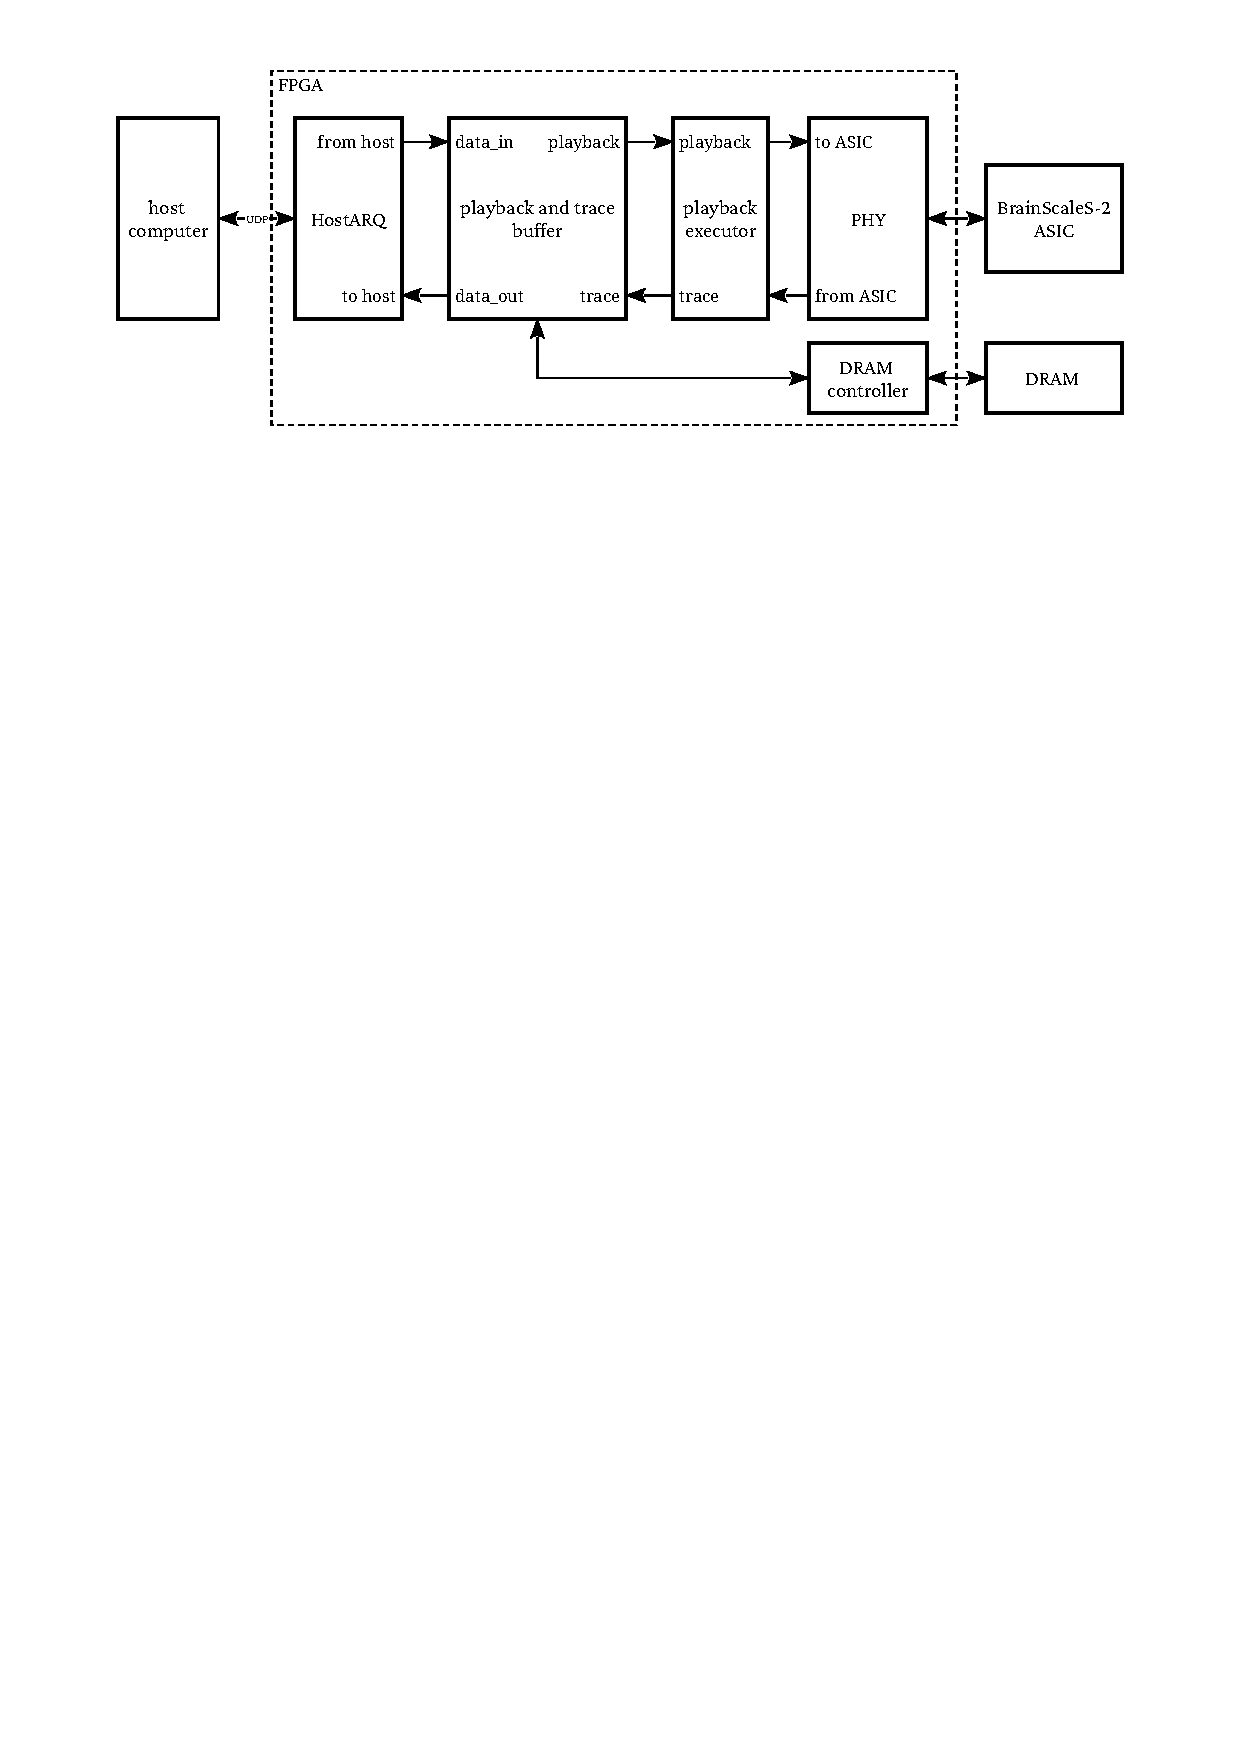
\includegraphics{diagrams/cropped/fpga_overview}}
\caption{Schematic overview of the FPGA design facilitating the communication between a network attached host computer and a HICANN ASIC}
\end{figure}

Communication with the \ASIC{} requires precise timing due to its physical nature, its emulation cannot be paused and resumed arbitrarily and a high data rate.
The high data rate interface of the \ASIC{} consists of eight pairs of \LVDS{} lanes, that can each operate at up to $\SI{2}{\giga\bit\per\second}$, for a total of $\SI{16}{\giga\bit\per\second}$ full duplex bandwidth.
To achieve the required precise timing a \FPGA{} is used to facilitate the communication between the host and the \ASIC{}.
Interaction with the \ASIC{} is converted into a sequence of instructions, the \PlaybackProgram{} that are processed by the \FPGA{} with deterministic timing at a resolution of $\SI{8}{\nano\second}$.
Data received from the \ASIC{} is timestamped with the same resolution by the \FPGA{}.

In the \BSSTwo{} system a \Xilinx{} \Kintex7{} \FPGA{} is used and the \LVDS{} lanes of the \ASIC{} are operated at $\SI{1}{\giga\bit\per\second}$.

The host and the \FPGA{} communicate using \UDP{} protocol over \Gigabitethernet{}. On top of \UDP{} the \HostARQ{}\autocite{ref:hostarq} protocol is used to implement a secured stream with a word size of \PhyWordSize{} over the unsecure \UDP{} protocol.

\subsubsection{Stream-Interfaces}
Many components of the \FPGA{} design are connected using stream interfaces. Throughout this thesis two different stream interfaces will be encountered. The first is \AXIStream{}\autocite{ref:axi_stream}, a standard interface used by many components provided \Xilinx{}.
\AXIStream{} is a unidirectional data stream, that connects a single master with a single slave. A \AXIStream{} consists of at least five signals:
\begin{itemize}
    \item \ACLK{} is the clock signal used by the stream. All other signals will be sampled on the rising edge of this clock.
    \item \ARESETn{} is the reset signal used by the stream. It is active low.
    \item \TDATA{} is the signal carrying the data. It is a multiple of eight bits wide and driven by the stream master.
    \item \TVALID{} is a single bit signal driven by the master indicating that valid data is present on the \TDATA{} signal.
    \item \TREADY{} is a single bit signal driven by the slave indicating that it can accept data.
\end{itemize}
The relation of \TDATA{}, \TVALID{} and \TREADY{} is governed by a set of rules. Data is transferred from the master to the slave when \TREADY{} and \TVALID{} are driven high simultaneously. This is called a two-way handshake mechanism.
Furthermore a master is not allow to wait for the slave to drive \TREADY{} high before asserting \TVALID{}. On the other hand, a slave is allowed to wait until the master drives \TVALID{} high until it drives \TREADY{} high.
When both the master and the slave can process the data fast enough, data can be transferred on every clock cycle. When this is the case \TREADY{} and \TVALID{} will be driven high continuously.
\AXIStream{} defines a set of further signals that can extend the functionality of this stream interface. In this thesis two optional signals will be relevant.
The first is \TKEEP{}. \TKEEP{} has one bit for every eight bits contained in the \TDATA{} signal and is driven by the master to indicate which bytes of the \TDATA{} signal contain valid data.
If bit $n$ of \TKEEP{} is driven high, bits $8n$ to $8(n + 1) - 1$ of \TDATA{} will contain valid data, if it is driven low the data contained in these bits is to be ignored by the slave.
The second optional signal is \TLAST{}. This is a single bit that is driven by the master which indicates that the current transfer is the last transfer of a packet.

The second stream type encountered in this thesis will be called \ValidNextStream{}. It is closely related to \AXIStream{}, but replaces the \TREADY{} signal with a \NEXT{} signal.
This is a single bit signal driven by the slave to indicate that the current data was processed and the master can present the next data word on \TDATA{}. Furthermore it has different rules regarding \TVALID{} and \NEXT{} compared to the rules of regarding \TVALID{} and \TREADY{}.
For a \ValidNextStream{} the master is allowed to wait until the slave drives \NEXT{} high before asserting \TVALID{}.

This different rule set means that in general a \AXIStream{} and a \ValidNextStream{} cannot be connected together by simply connecting the \TREADY{} and the \NEXT{} signals as they can deadlock. For example when connecting a \ValidNextStream{} master to a \AXIStream{} slave, the \ValidNextStream{} master is allowed to wait until the \AXIStream{} slave drives \TREADY{} (connected to \NEXT{}) until it drives \TVALID{}. However the \AXIStream{} slave is allowed to wait until \TVALID{} is driven high before asserting \TREADY{}. In this case both the slave and the master will wait forever and no progress will be made. This means when connecting a \ValidNextStream{} master to a \AXIStream{} slave, one has to use a \AXIStream{} slave that will assert \TREADY{} without waiting until \TVALID{} is asserted by the master.

\subsubsection{AXI}

\AXI{}\autocite{ref:axi} is standard communication bus used to connect some components of the \FPGA{} design. It is used to connect a single master to a single slave and is consists of a \ACLK{} and a \ARESETn{} signal that play the same role as they do in a \AXIStream{} as well as five independent channels:
\begin{itemize}
  \item The \AW{} channel transmits information about a write from the master to the slave. This information contains the address, the number of words that will be written (the \burstsize{}).
  \item The \AR{} channel transmits information about a read from the master to the slave. This information contains the address, the number of words that should be read (the \burstsize{}).
  \item The \W{} channel transmits the data that is written from the master to the slave.
  \item The \R{} channel transmits the data that is read from the slave to the master.
  \item The \B{} channel transmits a response that contains the result of a write from the slave to the master
\end{itemize}
Each of these channels uses the same handshaking signals \READY{} and \VALID{} as well as rules as a \AXIStream{}. Furthermore the \W{} and \R{} channels use a \LAST{} signal to indicate the last word of a burst.
Every channel operates separately from each other. This means that for example the data to be written can be transmitted by the master on the \W{} channel before the address information is transmitted on the \AW{} channel. A master is also allowed to transmit a second read on the \AR{} channel before having received the answer to the first.
From this it follows that the maximum data rate supported by the bus specification is a single data word each clock cycle on both the read and the write channels. Of course the actually data rate depends on the master and the slave.


\subsubsection{Playback Executor}
The \pbexec{} is responsible for processing the instruction stream that is received from the playback and trace memory management block as swell as receiving, time stamping and sending of events the trace stream events from the \ASIC{}.

The instructions that are processed by the executor can broadly be categorized into the three different categories of \readCat{}, \writeCat{}, \waitCat{}. Instructions of the \readCat{} category perform read operations on the several buses connected to the \pbexec{} and result result in response data that is sent to the trace stream in addition to the events from the \ASIC{}. Instructions of the \writeCat{} category perform writes to theses buses and instructions of the \waitCat{} are used to pause the processing of the instruction stream until a specific event takes place. This can for example be the elapsing of a specific duration or the completion of a read.

A special instruction, the \haltInstr{} is used to delineate separate experiments from each other. The \haltInstr{} marks the end of a \PlaybackProgram{} and looped back to the trace data where it can be used to differentiate trace data belonging to different \PlaybackProgram{}s.

The \pbexec{} operating at a \pbExecClock{} clock rate and can at most process a single instruction every clock cycle, however not every instruction can be processed in a single clock cycle. Obvious examples include instructions of the \wait{} category which purposefully pause the processing of the instruction stream. Similar to the instruction stream the \pbexec{} can also emit at most a single trace word every clock cycle.

% The maximum size of a playback instruction is $\SI{64}{\bits}$ which means

Both the playback instruction stream and the trace data are fundamentally a stream of variable size words. For transmission and reception over the fixed width \HostARQ{} streams they are encoded using \UT{} encoding scheme\autocite{ref:ut}.

For the playback instruction stream this encoding is performed on the host and on the \FPGA{} the \pbexec{} decodes the instruction stream before processing it.
Likewise the trace data generated / received by the \pbexec{} is encoded by the \pbexec{} before being sent to the trace stream.

The encoding and decoding also operates at a \pbExecClock{} clock rate and can produce / consume at most one \PhyWordSize{} sized word per clock cycle.

This means the maximum data rate at which the playback stream can be processed and the maximum data rate that is sent on the trace stream is
\[\PhyWordSize{} \pbExecClock{} = \pbExecBandwidth{}\]

\todo{write about arbitration priority}
\begin{figure}
\centerline{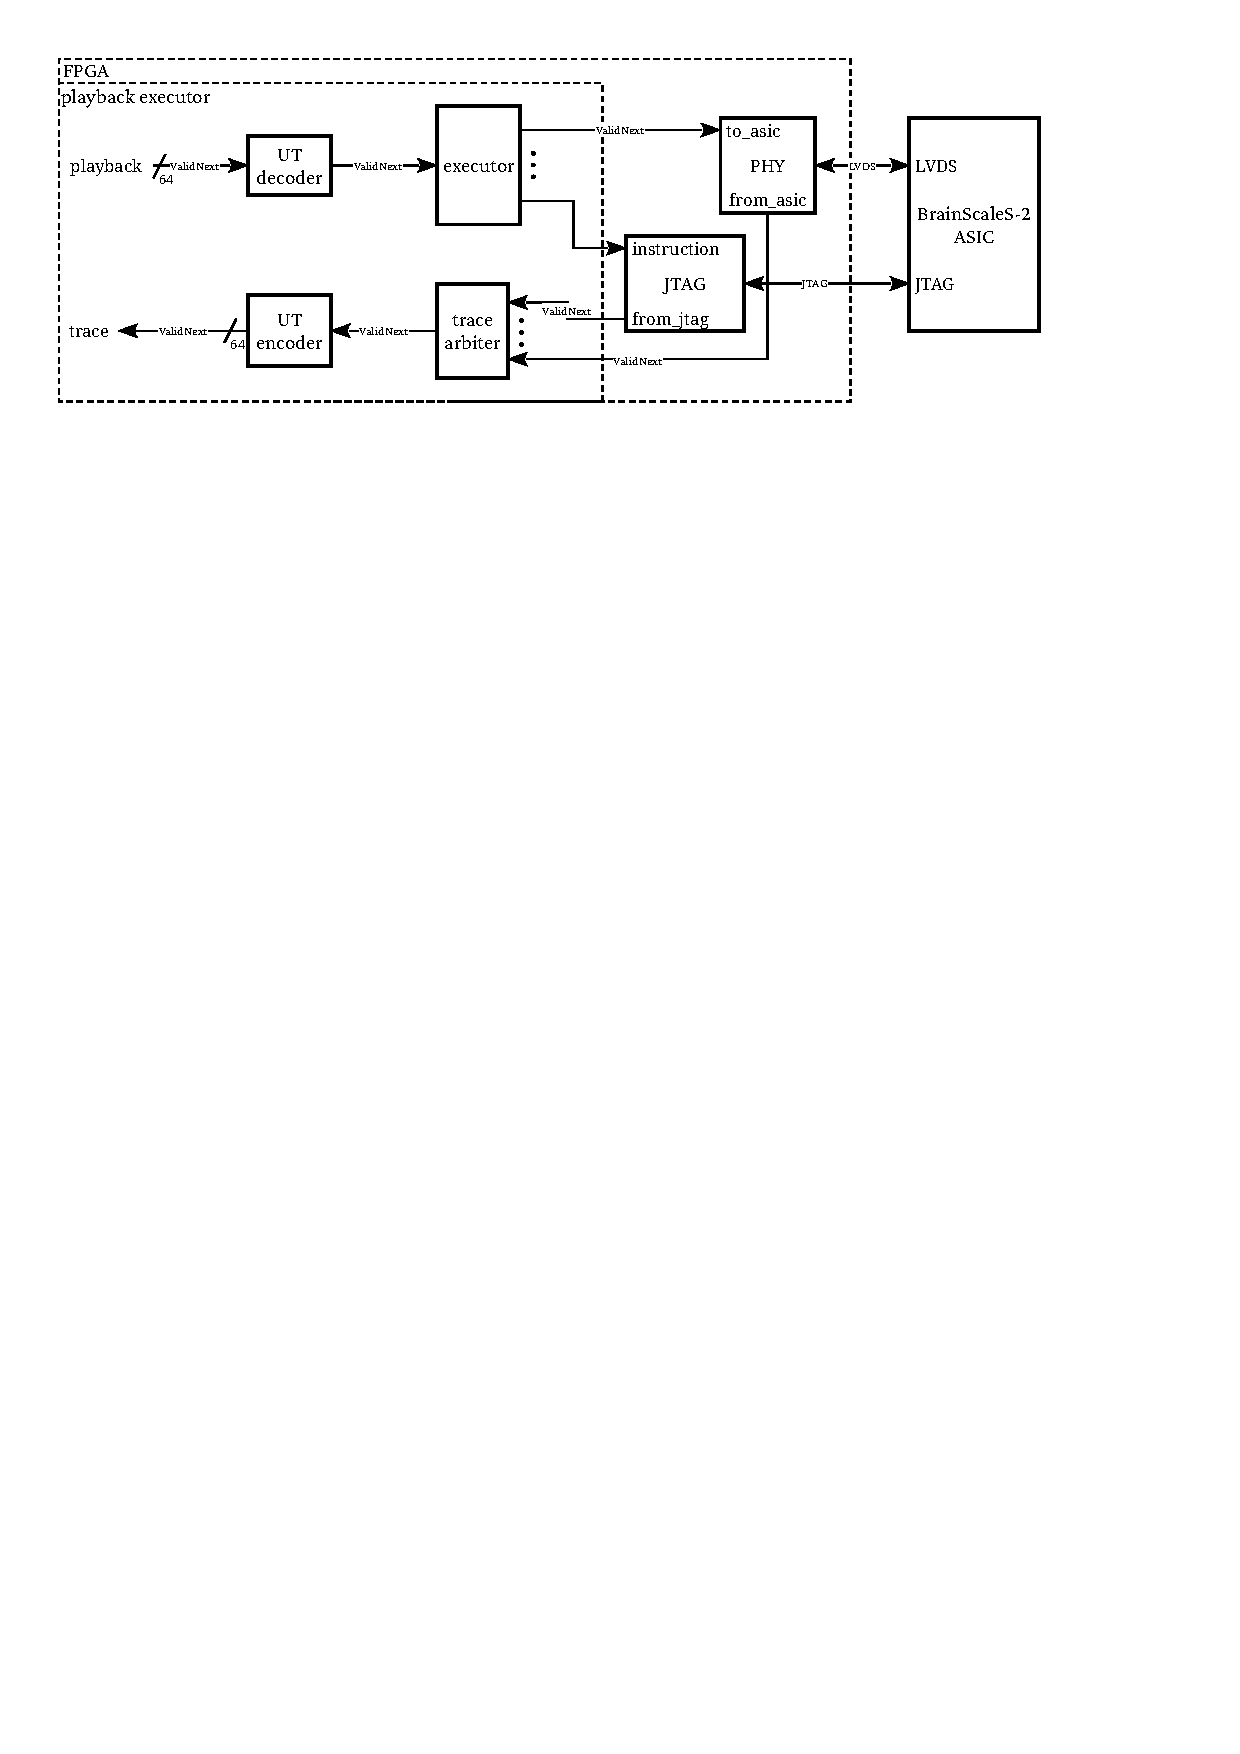
\includegraphics{diagrams/cropped/executor_detail}}
\caption{Overview of the \pbexec{}. This is on only a schematic representation and does not include all interfaces that the executor has access to and does not include all sources for trace data.}\label{diagram:executor}
\end{figure}

\subsubsection{Playback and Trace Memory Management}\label{sec:old-pb-trace-management}

The bandwidth between \FPGA{} and the \ASIC{} at \ASICBandwidth{} far exceeds the bandwidth between the host and the \FPGA{} of \HostBandwidth{}. To allow transmission and reception of the full data rate supported between the \FPGA{} and the \ASIC{} the \FPGA{} is connected to \SI{512}{\mebi\byte} of \DDR{} memory that is used as buffer for the playback and trace data. To interact with the \DDR{} memory the \XilinxMIG{} is used, configured to use a \AXI{} interface.

The playback and trace fifo management block responsible for storing the playback instructions stream received from the host into the \DDR{} memory and transmitting a complete experiment from the memory to the \pbexec{} as well as receiving the trace data from the \pbexec{} and storing it to the \DDR{} memory for later readout by the host.

In the current \FPGA{} design used by the \BSSTwo{} platform this block operates as a pair of \FIFO{}s. One for the playback stream and one for the trace stream. This \FIFO{} is implemented using the \Xilinx{} \VFIFO{} core, which implements a multi channel \FIFO{} backed by a \AXI{} accessible memory. It is connected to the \AXI{} interface of the \XilinxMIG{}. The \VFIFO{} core is used in a configuration using two channels. The first channel is used for the playback data and the second channel is used for the trace data.

The \pbmem{} block is responsible for scheduling the transmission of the playback instruction stream to the \pbexec{}.
It only allows data to be transmitted from the \VFIFO{} to the \pbexec{} when two conditions are fulfilled:
\begin{enumerate}
\item The \VFIFO{} channel for the playback data is empty or the \FIFO{} between the \VFIFO{} and the \pbexec{} is full
\item The \VFIFO{} channel for the playback data is full or a \haltInstr{} was written to the \VFIFO{} but not transmitted to the \pbexec{}
\end{enumerate}
When a complete \PlaybackProgram{} fits into the \VFIFO{} playback channel, these two conditions enforce that playback of the instructions that make up the \PlaybackProgram{} is only started once it was completely transmitted to the \VFIFO{}, as each \PlaybackProgram{} end with a \haltInstr{}. This ensures that the rate of instructions that can be transmitted to the \pbexec{} is not limited by the slow \HostARQ{} interface but instead by the \VFIFO{} and indirectly by the \XilinxMIG{} interface speed.
When a \PlaybackProgram{} does not fit completely in the \VFIFO{} playback channel, playback of it is started whenever the \VFIFO{} playback channel is full. This means that depending on rate the \pbexec{} is processing the playback instructions it is possible that the \HostARQ{} interface can be the limiting factor for the playback rate.
The \VFIFO{} is configured with a burst size of \(\SI{2048}{\byte}\) and using $\num{8192}$ $\SI{4}{\kibi\byte}$ allocated to each the playback and the trace channel, which means it can store at most \(\num{8192} · \SI{4}{\kibi\byte} = \SI{32}{\mebi\byte}\) per channel.

\begin{figure}
\centerline{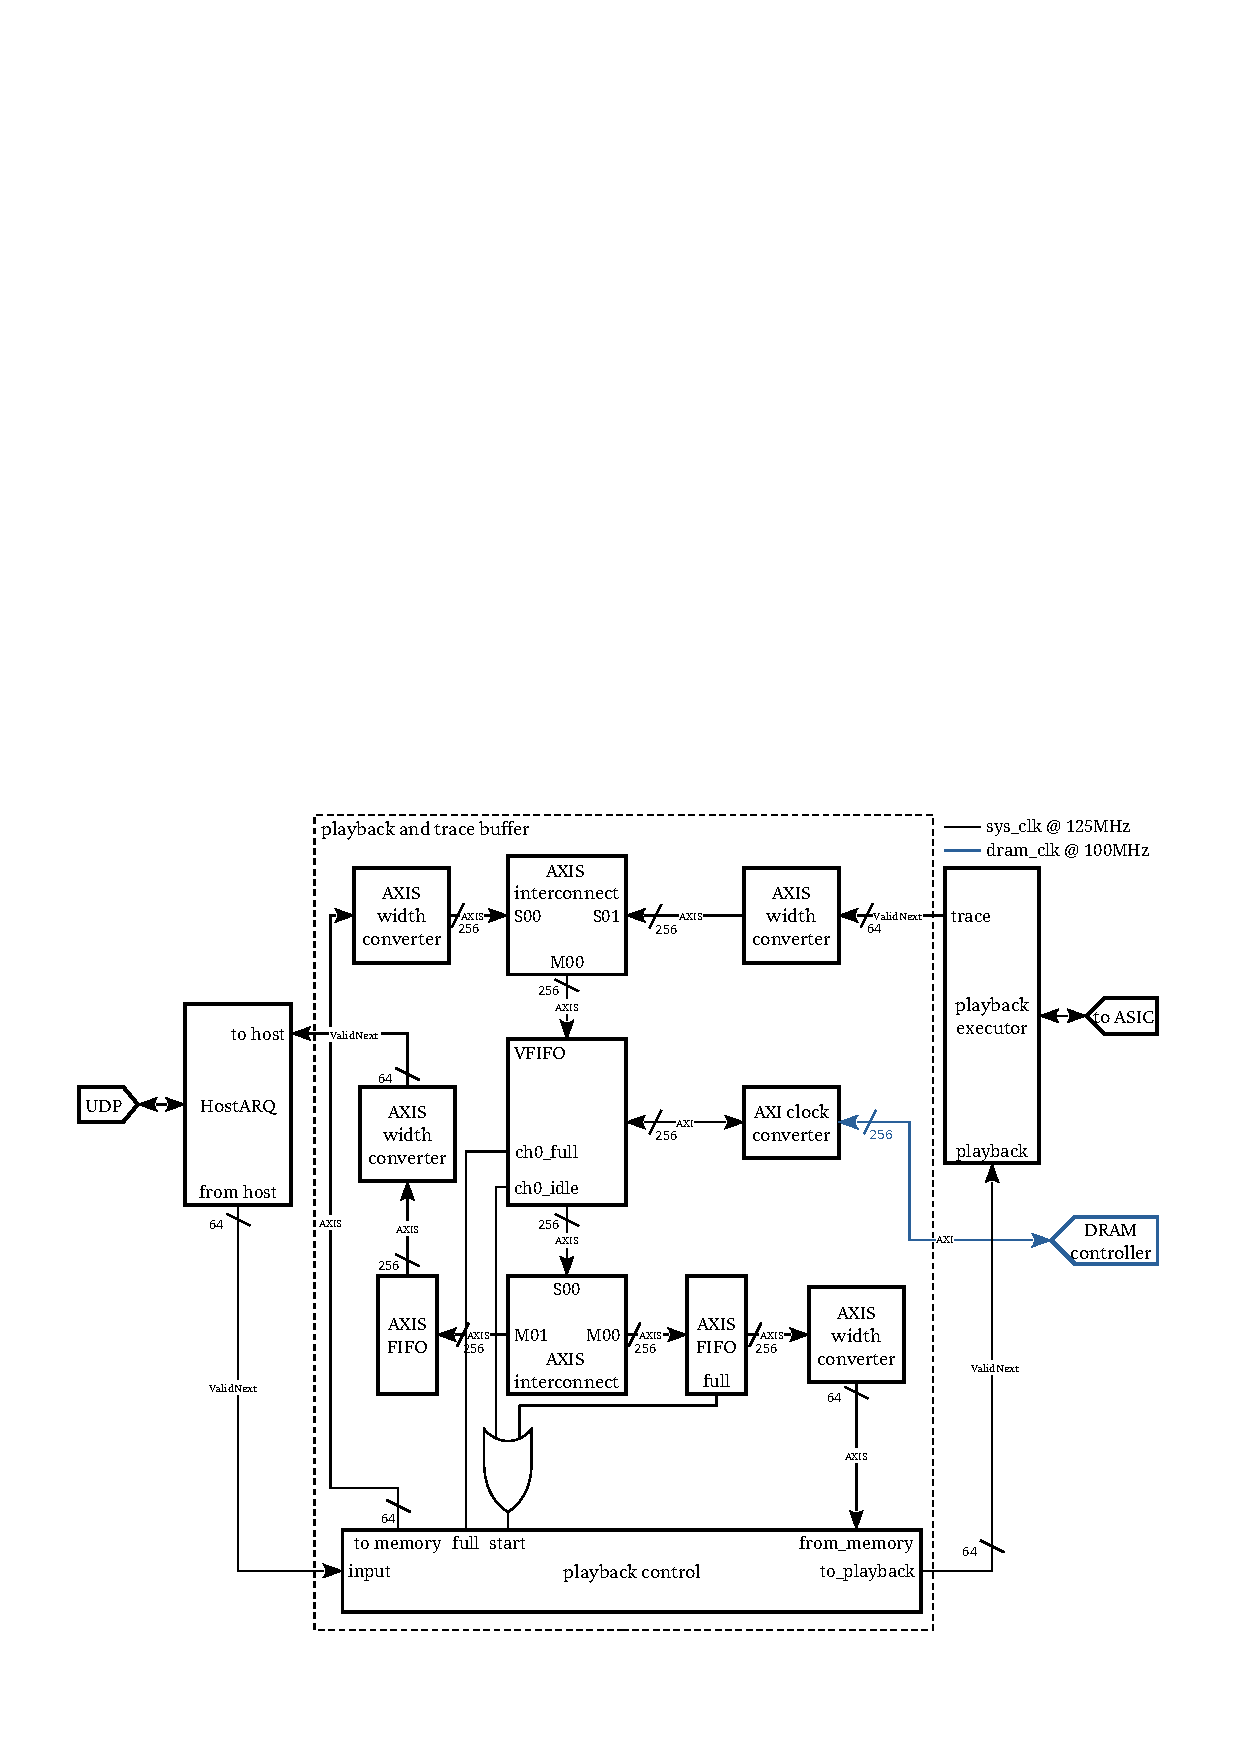
\includegraphics{diagrams/cropped/detail_old}}
\caption{Schematic overview of the old, FIFO-based, module handling the playback and trace data}\label{diagram:detail_old}
\end{figure}

This thesis will investigate a replacement for this \VFIFO{} based playback and trace memory management block.

\section{Implementation}\label{sec:impl}
To alleviate the shortcoming of the old playback and trace buffer design it is fundamentally redesigned.
There are four operations that need to be performed by the playback and trace buffer:
\begin{enumerate}
  \item Playback instructions sent by the host have to be written to the \DDR{} memory.
  \item The playback instructions received previously from the host have to transferred to the \pbexec{}.
  \item The trace data generated by the \pbexec{} has to be written to the \DDR{} memory.
  \item Trace data has to read from the \DDR{} memory and sent back to the host.
\end{enumerate}
These operations can be grouped into two categories: First host-side operations, which includes the first and the last of the four listed operations. The operations in this category allow the host to read and write the \DDR{} memory.
The second category is \FPGA{}-side operations, which includes the second and third operation listed. The operations in this category are responsible for reading and writing to the \DDR{} memory to generate the playback instructions stream for the \pbexec{} and to store the trace data generated by the \pbexec{}.
The first category of operations will be implemented using the \FAXI{} unit to allow memory mapped read and write access to the whole \DDR{} memory by the host.
To implement the second category of operations a scatter gather \DMA{} engine to on the one hand assembly the playback stream for the \pbexec{} from data that was written by the host to the \DDR{} memory and on the other hand to store the trace data transmitted by the \pbexec{} to the \DDR{} memory will be used

\autoref{fig:detail_new} shows a schematic overview of the replacement block developed in this thesis.

\begin{figure}[htbp]
\centerline{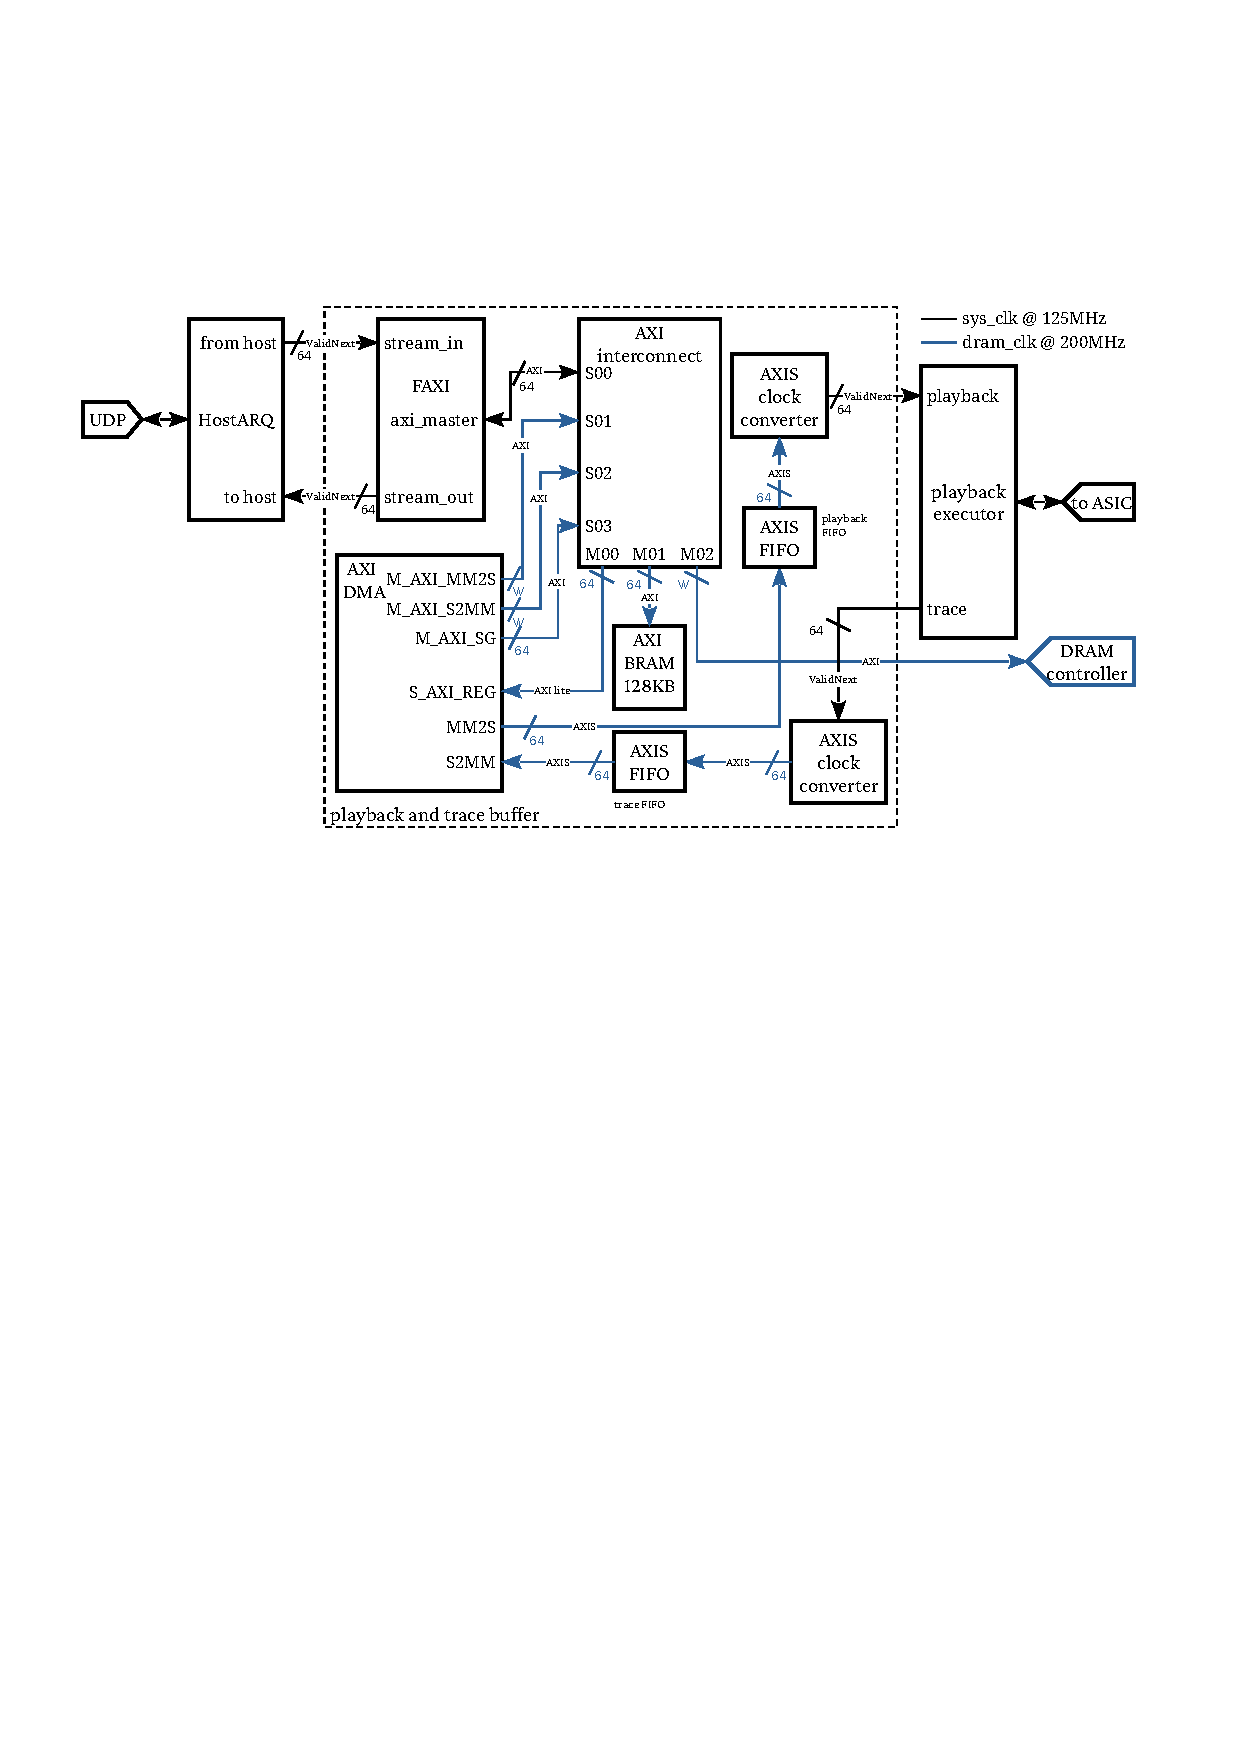
\includegraphics{diagrams/cropped/detail_new}}
\caption{Schematic overview of the new playback and trace buffer. Instead of implementing two \FIFO{}s it allows direct read and write access to the \DDR{} memory by the host. A scatter gather \DMA{} engine is used to read from the \DDR{} memory and transmit the read data as the playback stream to the \pbexec{} as well as writing the trace data from the \pbexec{} to the \DDR{} memory.}\label{fig:detail_new}
\end{figure}

\subsection{FAXI}
To allow the host to read and write to the \DDR{} memory the \FAXI{} unit is used. This unit was developed by the Electronic Vision(s) group for a different \FPGA{} design. It implements a bridge between the \HostARQ{} \FPGA{} interface of two \PhyWordSize{} wide streams and an \AXI{} Subordinate with data width of \PhyWordSize{} and an address size of \PhyWordSize{}.
Read and write requests are encoded in the \HostARQ{} stream using a \PhyWordSize{} header controlling the kind of operation (read or write) and the \burstsize{}. This header is followed by a \PhyWordSize{} address and for a write requests by the specified number of \PhyWordSize{} words.
Read data and write response is sent back to the host following a similar scheme of a \PhyWordSize{} header followed by the read data words.
Finally, \FAXI{} supports a \globalfence{} operation, that blocks the processing of the further data until every outstanding read or write transaction is completed.

The subset of \AXI{} that is supported by it is summarized in \autoref{tbl:faxi_axi_features}.

\begin{table}
  \begin{center}
\begin{tabular}{ll}
  \toprule
  feature & status  \\
  \midrule
  data width & $\SI{64}{\bit}$ \\
  address width & $\SI{64}{\bit}$ \\
  transaction ID & not supported \\
  AxLOCK & not supported \\
  AxCACHE & not supported \\
  AxPROT & not supported \\
  AxQOS & not supported \\
  AxREGION & not supported \\
  user signals & not supported \\
  narrow transfers & not supported \\
  write strobe & partially, see description \\
  \bottomrule
\end{tabular}

  \end{center}
\caption{Summary of the \AXI{} features supported by \FAXI{}. \AXI{} usually allows a different write strobe for each data word of a write transaction. \FAXI{} only allows a fixed write strobe for a complete write transaction.}\label{tbl:faxi_axi_features}
\end{table}

\HostARQ{} is configured to use a maximum packet size of $\num{180}$ words with $\PhyWordSize{}$ per words.
Each packet has an overhead of $\SI{78}{\byte}$ from the \Gigabitethernet{}, IPv4, \UDP{} and \HostARQ{}.
The maximum burst length of an \AXI{} write is $\num{256}$ words and to encode a write-burst \FAXI{} has an overhead of two $\PhyWordSize{}$ words (the header and the address). From the maximum data rate $\SI{1}{\giga\bit\per\second}$ of \Gigabitethernet{} one obtains for the maximum write bandwidth possible
\[
B_{\text{\FAXI{},w}} = \num{180} · \PhyWordSize{} \frac{\SI{1}{\giga\bit\per\second}}{\SI{78}{\byte} + 180 · \PhyWordSize{}} · \frac{256 \PhyWordSize{}}{(256 + 2) \PhyWordSize{}} \approx \SI{112.21}{\mebi\byte\per\second}
\]
For a read the overhead due to the \FAXI{} encoding is only one \PhyWordSize{} word and one obtains
\[
B_{\text{\FAXI{},w}} = \num{180} · \PhyWordSize{} \frac{\SI{1}{\giga\bit\per\second}}{\SI{78}{\byte} + 180 · \PhyWordSize{}} · \frac{256 \PhyWordSize{}}{(256 + 1) \PhyWordSize{}} \approx \SI{112.64}{\mebi\byte\per\second}
\]


\subsection{AXIDMA}\label{sec:AXIDMA}
The \AXIDMA{} IP core by \Xilinx{}\autocite{ref:axidma} provides a \DMA{} engine. This is split into two separate channels, the \MMToS{} channel and the \SToMM{} channel.
The \MMToS{} channel is used to read data from an \AXI{} Subordinate and transmit the data using an \AXIStream{}. It is used to read the data written to the \DDR{} memory by the host using \FAXI{} and transmit it to the \pbexec{}. The \SToMM{} channel performs the opposite operation and writes data from an \AXIStream{} to an \AXI{} Subordinate. It is used to write the trace data received from the \pbexec{} to the \DDR{} memory.
Moreover, the \AXIDMA{} core has a separate set of \AXILite{} accessible registers that are used to control its operation.

The \AXIDMA{} \DMA{} engine can be used to perform scatter and gather operations. In the scatter gather mode the operation of these channels is controlled using a chain of \descriptor{}s.
Each \descriptor{} contains an address, a buffer length, the address of the next descriptor, as well as a status and a control field. For the \MMToS{} channel, the address specified in the descriptor is the address of the first byte that is read by the channel. The total number of consecutive bytes read from this address is specified by the buffer length. When every byte specified by the descriptor was read, the \AXIDMA{} sets the completed flag in the status field and, the next descriptor as specified by the next descriptor address is used to continue the operation. The control field contains a start and an end of frame flag. The latter is used to generate the \TLAST{} signal of the \AXIStream{} driven by the \MMToS{} channel. Operation of the \MMToS{} channel is started by writing the address of the first descriptor and the address of the last descriptor to the \curdesc{} and \taildesc{} registers of the \MMToS{} channel.

The \SToMM{} channel operates similarly. For each descriptor it writes up to the specified buffer length consecutive bytes from the \SToMM{} \AXIStream{} Receiver to the address specified in the descriptor.
Whenever the last word of a packet as specified by the \TLAST{} signal or the number of bytes specified by the buffer length was written, the completed flag as well as the number of transferred bytes is updated in the status field of the descriptor and the next descriptor is read from the specified address for the next descriptor.

The \AXIDMA{} core uses separate \AXI{} Managers for the \SToMM{} and the \MMToS{} channel as well as the scatter gather descriptors.

\subsection{New playback and trace buffer}
Using an \AXI{} interconnect like the \smartconnect{} allows operations from multiple \AXI{} Managers to be multiplexed to multiple \AXI{} Subordinates based on the address.
For the playback and trace buffer design it is used to allow access from \FAXI{} and both \AXIDMA{} channels to the \AXI{} interface of the \DDR{} controller.
\autoref{tbl:axi_memory_map} contains an overview of the memory map that was chosen. The interconnect is used to allow \FAXI{} to access the \DDR{} memory, the \AXIDMA{} registers and the scatter gather descriptor memory while also allowing both \AXIDMA{} channels to access the \DDR{} memory and \AXIDMA{} to access the scatter gather descriptor memory.

To store the scatter gather descriptors there are two options. One could use the main \DDR{} memory or a separate memory. Using a separate memory has several advantages. It ensures that interaction such as reading and writing the \descriptor{} cannot have any effect on the reads and writes to the \DDR{} memory performed by the \SToMM{} and \MMToS{} channels. Additionally, reads and writew to it have a lower latency than reads and writes to the \DDR{} memory.
Each \descriptor{} has a size of $\SI{64}{\byte}$, accordingly the $\SI{128}{\kibi\byte}$ memory used for the descriptors allows for up to $\num{2048}$ descriptors.

\begin{table}
\begin{center}
\begin{tabular}{llr}
\toprule
  \AXI{} Subordinate & address & size \\
  \midrule
  \DDR{} memory & $\texttt{0000\,0000}_{16}$ & \DDRSIZE{} \\
  scatter gather descriptor memory & $\texttt{A000\,0000}_{16}$ & $\SI{128}{\kibi\byte}$ \\
  \AXIDMA{} registers & $\texttt{B000\,0000}_{16}$ & $\SI{8}{\kibi\byte}$ \\
  \bottomrule
\end{tabular}
\end{center}
\caption{\AXI{} memory map.}\label{tbl:axi_memory_map}
\end{table}

As every address that is accessible according to the address map given in \autoref{tbl:axi_memory_map} can be represented with $\SI{32}{\bit}$ an address width of $\SI{32}{\bit}$ is used every \AXI{} bus.
The \AXIDMA{}, \XilinxMIG{}, \smartconnect{} and the \AXIBRAMController{} do not have an fixed \AXI{} data width but instead allow a variety of different configurations.
Their configuration was chosen to use the minimal width that satisfy the requirement of $\pbExecBandwidth{}$ bandwidth for the playback and the trace stream generated by the \MMToS{} and \SToMM{} channels. Minimizing the width directly reduces the required amount of \FPGA{} resources like \LUT{}s and \FF{}s and moreover reduces the number of routing resources. The \FPGA{} design is limited by these routing resources\autocite{ref:fpga_routing_limited}.
As described in \autoref{sec:AXI} the theoretical maximum data rate of an \AXI{} bus is determined by the clock frequency and the data width.

There are three choices for the clock
\begin{enumerate}
    \item The $\SI{125}{\mega\hertz}$ clock shared by the \HostARQ{} and the \pbexec{}.
    \item The same clock as the \XilinxMIG{} memory interface.
    \item A clock not shared with any of the ports
\end{enumerate}
The second option was selected with the \XilinxMIG{} operating in 2:1 mode resulting in a clock frequency of $\SI{200}{\mega\hertz}$. Using the 2:1 mode instead of the 4:1 mode with a clock frequency of $\SI{100}{\mega\hertz}$ halves the required data width as the clock frequency is doubled. For the same region using the $\SI{200}{\mega\hertz}$ was preferred over the $\SI{125}{\mega\hertz}$ clock of the \HostARQ{} and \pbexec{} interfaces.
% \todo{maybe something about how it actually manages to implement them at 200mhz and we therefore do not need to use a slow clock domain?}
Furthermore, using a clock that is shared with some ports of the module reduces the required clock domain crossing logic.

The \SToMM{} an \MMToS{} \AXIStream{}s are configured to use a data width of \PhyWordSize{}. At clock frequency of $\SI{200}{\mega\hertz}$ this results in a bandwidth of $\SI{12.8}{\giga\bit\per\second}$, satisfying the minimum requirement of \pbExecBandwidth{}. By choosing the same data width the \pbexec{} playback and trace streams no width conversion is necessary. For the bandwidth that can actually be achieved by the \AXIDMA{} only limited information is provided by \Xilinx{}. \Xilinx{} specifies that an \AXIDMA{} operating at a clock frequency of $\SI{100}{\mega\hertz}$ is able to achieve $\SI{99.76}{\percent}$ of the theoretical throughput on the \MMToS{} channel and $\SI{74.64}{\percent}$ of the theoretical throughput on the \SToMM{} channel when transferring $\SI{10000}{\byte}$\autocite{ref:axidma}. Assuming the relative throughput is independent of the clock frequency operation a $\SI{200}{\mega\hertz}$ should be able to achieve a bandwidth greater than the requirement of $\pbExecBandwidth{}$.

For the data width $W$ of the remaining \XilinxMIG{} \AXI{} Subordinate interface and the \SToMM{} and \MMToS{} \AXI{} Manager a choice of \PhyWordSize{} and $\SI{128}{\bit}$ is evaluated.

\Xilinx{} specifies that the bandwidth achievable by the \XilinxMIG{} will vary depending on the access pattern and other system parameters. It is of course limited by the maximum bandwidth that is achievable using the \DDR{} interface of the memory. An upper bound of this bandwidth $B_{\text{\DDR{}}}$ can be determined from the clock frequency the memory is operated at $f_{\text{\DDR{}}} = \SI{400}{\mega\hertz}$ and the number of data lanes $n_{\text{dq}} = \num{32}$
\[B_{\text{\DDR{}}} = 2 f_{\text{\DDR{}}} n_{\text{dq}} · \SI{1}{\bit} = \SI{25.6}{\giga\bit\per\second}\]
This upper bound is not strict, it can not be reached continuously due to the operations required by the \DDR{} protocol like refresh pauses and row pre-charging time\autocite{ref:ddr3_standard}. As \DDR{} operates in a \halfduplex{} fashion, this bandwidth is shared by both reads and writes to the memory. This yields an efficiency necessary to satisfy the full bandwidth on both the trace and the playback channel of
\[\frac{2 · \pbExecBandwidth{}}{B_{\text{\DDR{}}}} = \SI{62.5}{\percent}\]

Finally, three different choices for the \SToMM{} and \MMToS{} \FIFO{}s are evaluated
\begin{itemize}
\item No \FIFO{}.
\item A packet mode \num{256} word \FIFO{} for the \MMToS{} \AXIStream{}. A packet mode \FIFO{} will only transmit data on its Transmitter interface if it is full or it contains at least one whole packet, as signaled by the \TLAST{} signal. This \FIFO{} is labeled \texttt{playback FIFO} in \autoref{fig:detail_new}.
\item A packet mode \num{256} word \FIFO{} for the \MMToS{} \AXIStream{} and a \num{256} word \FIFO{} for the \SToMM{} stream. This \FIFO{} is labeled \texttt{trace FIFO} in \autoref{fig:detail_new}.
\end{itemize}

Guided by measurements of the actually achieved bandwidth on the trace and the playback streams as described in \autoref{sec:pb_trace_verif} and \autoref{sec:pb_trace_bw} the data width $W$ is chosen to be $\SI{128}{\bit}$ and both, the \texttt{playback FIFO} and the \texttt{trace FIFO} are included.

Lastly note that in this case the \ValidNextStream{} Transmitter of the \pbexec{} used for the trace stream can be directly connected to the \SToMM{} \AXIStream{} Receiver, as the \SToMM{} \AXIStream{} Receiver does not wait for a \TVALID{} signal until it asserts \TREADY{}.


% \todo{tie back the choices to the diagram}
% \todo{write 256 x 64 = 18k = 1 bram?}

% \todo{talk about why valid next and axi stream are compatible here}
% \todo{write about bandwidth of mig and axidma}

\subsection{Theory of operation}
The old playback and trace buffer design was used by the host for sending the \PlaybackProgram{}s that it wants to execute to the \FPGA{} and then receiving the resulting trace data.
The new design requires more steps to execute a set of \PlaybackProgram{}s and receive the generated trace data.
First, the host writes the playback instructions corresponding to a \PlaybackProgram{} that should be executed to the \DDR{} memory using the \FAXI{} block. It does not have to place the instructions into one contiguous region of the memory but instead can split the instructions into multiple regions.
To execute the playback instructions the host writes a \descriptor{} chain to the scatter gather descriptor chain memory that instructions the \AXIDMA{} to read the (potentially multiple) regions belonging to each \PlaybackProgram{} in the correct sequence.
Furthermore, the host creates a chain of \descriptor{} that is used by the \SToMM{} channel to store the received trace data in unused regions of the \DDR{} memory.

The old playback and trace buffer design sends back the trace data to the host as soon as trace data is generated. To separate which trace data was received for which \PlaybackProgram{} the host then uses the \haltInstr{} at the end of each \PlaybackProgram{} which is looped back to the trace data once it is executed by the \pbexec{}.
In this new design readout of the trace data has to be initiated by the host. The host can determine the number of received bytes from the status fields of the \descriptor{} chain used for the trace data.
However, the \completed{} flag and the number of received bytes stored in the status field of a \descriptor{} used by the \SToMM{} channel is only updated under two circumstances. It is updated, when the number of bytes written matches the configured buffer length or when the \SToMM{} channel receives a whole packet (as signaled by the \TLAST{} signal). In general the trace \descriptor{} chain cannot be configured to contain exactly the number of bytes used by the trace data, as the amount of trace data that is generated cannot be known ahead of time in general, so the \TLAST{} signal has to be used to control the \SToMM{} channel to switch to the next \descriptor{} and update the status field.
The \UTEncoder{} used by the \pbexec{} to generate the fixed word width trace data stream has therefore be extended to support the \TLAST{} signal so that the \TLAST{} signal can be generated by the \pbexec{} whenever a \haltInstr{} is added to the trace stream.

After the host has written the \descriptor{} chain for the playback and the trace data, it starts the execution of the \PlaybackProgram{} configuring the \SToMM{} and the \MMToS{} channel with the correct \descriptor{}s.
By polling the status field of the trace data descriptors the host waits for every \PlaybackProgram{} was executed and finally reads the generated trace data.

As outlined in this section to execute \PlaybackProgram{}s and receive their result there are substantially more steps required than with the new design for the playback and trace buffer than the old. The most significant difference is that the transmission of the trace data from the \FPGA{} and to the host is not started as soon as it is generated, but instead only when a \PlaybackProgram{} is finished. This can potentially significantlyl increase the experiment runtime for certain experiments. This disadvantage will be further analyzed in end of \autoref{sec:ayo} and in \autoref{sec:rate}. Finally \autoref{sec:latency_reduction} will outline possible future extensions of this new design to alleviate this disadvantage.
\subsection{ayo --- AXI Memory Orchestrator}\label{sec:ayo}
The \FPGA{} design is only one part of the tools required to perform experiments using the \HICANNX{} \ASIC{}. On the host computer side a set of layered software components are used for the description and execution of experiments. These software components follow a layered approach with layers exposing an increasingly more abstract interface to their users. A detailed description of this software stack can be found in \autocite{mueller2022scalable}.

To use the new playback and trace buffer described in this thesis changes to this software stack are required. These changes can be categorized into to two different categories
\begin{enumerate}
\item Changes that are required because the operations that need to be performed by the host to execute a \PlaybackProgram{} on  an \FPGA{} and to receive the resulting trace data have changed. For example the host has to program the \AXIDMA{} block correctly and needs to use the \FAXI{} block to read and write to the playback and trace memory.
\item Changes that allow the software to make use of the new features made possible by this new playback and trace buffer. This includes the ability to reuse (parts) of an already transmitted \PlaybackProgram{} and partial readout of the received trace data.
\end{enumerate}

In this thesis only the changes falling into the first category are performed. Changes that fall into the second category are prepared by making the lower level \API{} more flexible, however these additional features are not exposed to the higher levels. The changes belonging to the first category are implemented by extending the \BSSTwo{} software architecture with an additional layer in the communication category, \ayo{} (Axi memorY Orchestrator) that is responsible for communication using the \FAXI{} interface and the configuration of the \AXIDMA{} block. \autoref{fig:bss_stack} shows an overview of the software stack and the loction of this new \ayo{} layer. The \ayo{} layer is used by the \hxcomm{} library. \hxcomm{} is used by the higher level software to run a single \PlaybackProgram{} and retrieve the trace data that is generated for them. It is responsible for the \UT{} encoding of the playback instructions and \UT{} decoding of the trace data as well as the abstraction of the different backends for communication with either the actual hardware or a simulation of the hardware.

\begin{figure}[htbp]
\centerline{\inputtikz{diagrams/bss2stack}}
\caption{Schematic overview of the \BSSTwo{} software architecture. In this thesis it was extended by the \ayo{} component marked in magenta. Figure modified from \autocite{mueller2022scalable}}\label{fig:bss_stack}
\end{figure}

\autoref{listing:ayo_interface} gives an overview over the main \API{} of \ayo{}. The \code{alloc} function is used to reserve a region of memory that is big enough to hold the specified number of \code{bytes}. This function returns an opaque \code{Handle} that is used by the \code{free} function, which marks the region as unused again as well as the \code{read} and \code{write} functions that are used to read and write from the memory region corresponding to the \code{Handle}.
Finally, the \code{run} is used to schedule the execution of one or more \PlaybackProgram{}s. The list of \code{playback_regions} defines the order and the location of the parts of the \PlaybackProgram{}s, that will be sent to the \pbexec{}, while the list of \code{trace_regions} contains a list of memory regions that is used for the trace data. The \code{RunResult} returned by this function is used to query the status of the execution as well as read back of the trace data.

With the modifications performed in this thesis \hxcomm{} uses only a subset of the functionality provided by the \ayo{} layer and the interface of \hxcomm{} is not modified. Accordingly, all higher software levels can use this new playback and trace buffer design without any changes.
The interface of \hxcomm{} allows exactly one \PlaybackProgram{} to be executed and its trace data to be received. With \ayo{} this is performed by simply allocating two memory regions, one that contains the whole \PlaybackProgram{} and a second one that covers the rest of the available memory for the trace data. The \PlaybackProgram{} is written to the playback and trace memory using \code{write} and afterwards the \PlaybackProgram{} is executed by using the \code{run} function with exactly one playback and one trace region. Finally, the received trace data is read and transmitted to the higher level.

\begin{listing}
\begin{minted}{c++}
using axi_word_t = uint64_t;
class AYO
{
	Handle alloc(ddr3_size_t bytes);

	void free(Handle handle);

	std::future<WriteResult> write(Handle target, std::vector<axi_word_t> words);

	std::future<std::vector<axi_word_t>> read(Handle target);

	RunResult run(std::vector<WriteResult> playback_regions, std::vector<Handle> trace_regions);
};

class RunResult {
	void wait();
	std::future<std::vector<axi_word_t>> read();
	std::future<Status> status();
	std::vector<Result> traces();
	std::vector<Result> playback_programs();
}

class Result {
	void wait();
	std::future<std::vector<axi_word_t>> read();
	std::future<SingleStatus> status();
}
\end{minted}
\caption{Overview of the interface presented by \ayo{}. It was simplified for brevity.}\label{listing:ayo_interface}
\end{listing}

Internally the \code{run} functions converts the list of playback and trace memory regions into a playback and a trace descriptor chain. Consecutive playback regions are merged and each resulting playback and trace memory region is described using at least one \descriptor{}. Regions that are longer than the maximum buffer length of $\SI{67108863}{\byte}$ that can be specified in a \descriptor{} are converted into multiple descriptors. The \descriptor{} chains for the playback region are linked together in the same order as they were given to the \code{run} function, the same applies to the \descriptor{} chains for the trace regions. Consecutive trace regions are not merged together, as every \PlaybackProgram{} needs at least one trace descriptor, due to the \haltInstr{} ends a \PlaybackProgram{} causing the \AXIDMA{} to switch to the next trace descriptor as described previously.
\autoref{fig:ayo_chain_detail} shows a schematic overview of how the descriptor chains are created by the \code{run} function.

\begin{figure}[htbp]
\centerline{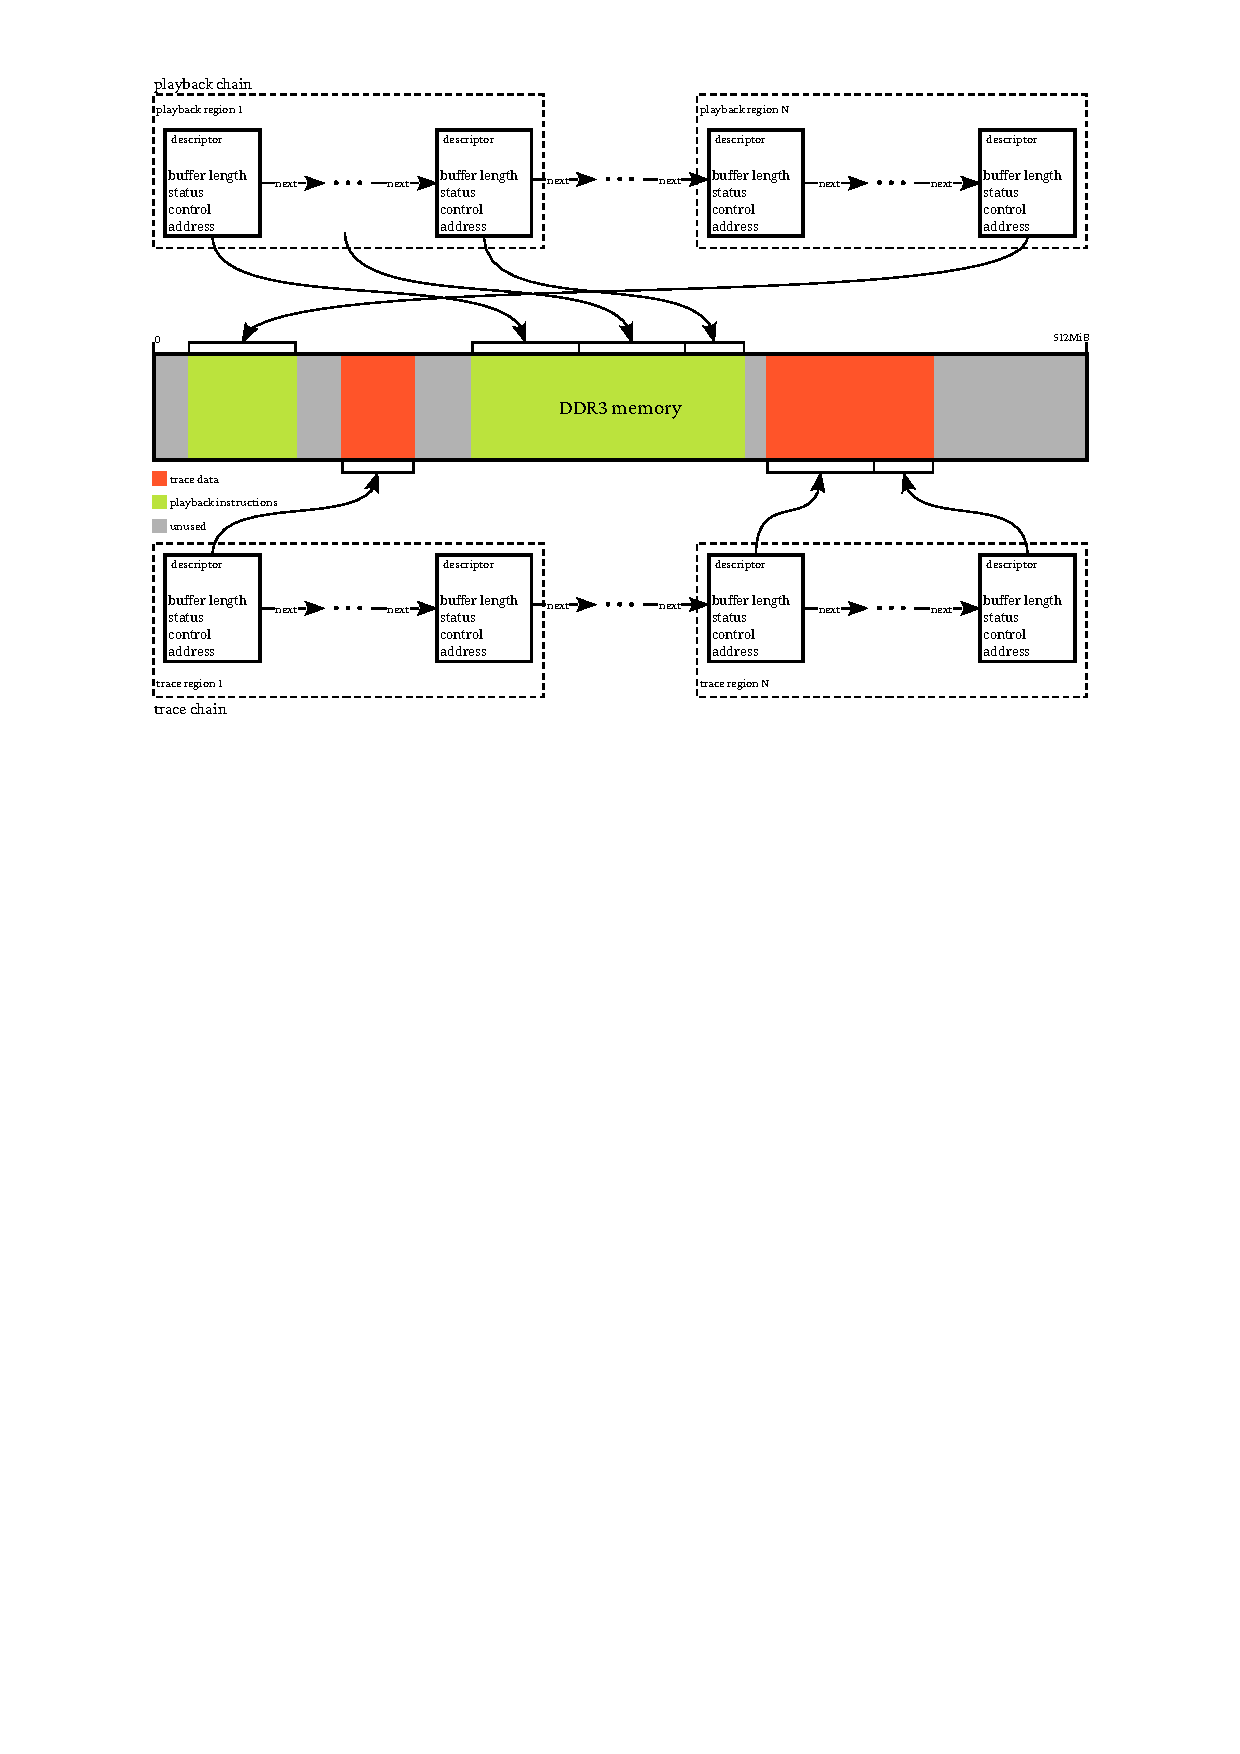
\includegraphics{diagrams/cropped/ayo_chain_detail}}
\caption{Schematic overview of an example for the playback and trace descriptor chains created for a set of playback and trace regions. In this example two playback regions were specified. The first playback region contains more than twice the maximum permissible buffer length for a single \descriptor{} and is therefore converted into a chain of three descriptors. The second playback region is small enough for one \descriptor{} to be sufficient. Note that the first playback region is stored after the second in the memory, but due to the order of the playback descriptors, the first playback region will be transmitted to the \pbexec{} before the second one. This example also has two trace regions, the first being small enough to be described by a single \descriptor{} and the second needing two \descriptor{}s. The order of the playback and trace regions in the \DDR{} memory is independent of the order they are actually used in.}\label{fig:ayo_chain_detail}
\end{figure}

The rate of experiments that can be performed in a \HWinTheLoop{} style operation, where each \PlaybackProgram{} depends on the trace data of the previous \PlaybackProgram{} is expected to be limited mainly by the round trip time between the host and the \FPGA{}. The old playback and trace buffer design requires just one round trip from the host to the \FPGA{}. It sends the \PlaybackProgram{} and then receives the trace data as it is generated.
To perform a single experiment with the new playback and trace buffer design five steps need to be performed
\begin{enumerate}
    \item\label{step:exec_first} The \PlaybackProgram{} is written to the \DDR{} memory
    \item A descriptor{} chain for the \PlaybackProgram{} and the memory region that captures the trace data is written to the \descriptor{} memory
    \item\label{step:exec_third} Operation of the \SToMM{} and \MMToS{} channels of the \AXIDMA{} is started by writing the proper \descriptor{} chain addresses to the \curdesc{} and \taildesc{} descriptors.
    \item The status field of the \descriptor{}(s) for the trace data is polled to determine when the \PlaybackProgram{} has finished execution as well as the size of the generated trace data.
    \item The trace data is read from the \DDR{} memory.
\end{enumerate}
The first two steps need to be completed before the third step is performed to guarantee both the playback and the descriptor data was written before it is read by the \AXIDMA{} unit.
A naive implementation would wait for the reception of the write response for the first two steps until it continues with the third step, but using the special \globalfence{} operation of the \FAXI{} block \ayo{} does not have to wait for response to the write operations in steps \autoref{step:exec_first} to \autoref{step:exec_third} and can instead ensure the write operations for the first two steps was completed before the \AXIDMA{} unit will be configured and in turn the data written in the first two stes will be read by the \AXIDMA{} by inserting a \globalfence{} operation before the write operations that configure the \AXIDMA{}. It is however unavoidable to wait for the response to the read operations that poll the status field of the trace \descriptor{}s, as the response data is used to determine when the readout of the trace data can be started as well as determining the size of the generated trace data. For an experiment with a single trace descriptor the lowest number of round trips that are necessary is therefore the number of times the status field has to be read until the \PlaybackProgram{} is completed plus one round trip for the readout of the trace data yielding a minimum of two round trips.
Accordingly, in the case of \HWinTheLoop{} style operation with small \PlaybackProgram{}s it is expected that the rate of experiments is at most half of the rate that can be achieved with the old playback and trace buffer design.
Future extensions of the playback and trace buffer design could reduce the number of roundtrips required again, by for example introducing a separate channel for the trace data, that bypasses the trace buffer and directly sends the trace data to the host.
\subsubsection{Allocator}
With the old FIFO based system, the \VFIFO{} module in the \FPGA{} is responsible for placing the playback data in the \DDR{} memory, reading it again from the address it was placed at, and vice versa for the trace data.
Changing the host interface to be memory mapped instead of FIFO based shifts the responsibility deciding the placement of the playback and trace data from the \FPGA{} to the host.
Furthermore, the playback data is no longer accessed in a strictly FIFO way, but instead can be built up from multiple blocks, with some blocks potentially being used by multiple experiments.
Management of the memory is abstracted by \ayo{} which simply presents the higher layers with the \code{alloc} and \code{free} functions that are used to reserve regions of memory and mark them as unused again.
In the \ayo{} layer tracking which regions of memory are already used for playback or trace data as well as allocating new regions or marking previously used regions as unused is done by an \allocator{}, which in turn provides the address for each of the memory regions. Its interface is described in \autoref{listing:allocator_interface}.

On creation, the allocator is given the size of the memory used for the playback and trace. Its \code{alloc} function finds an unused region in the memory that has at least a size of \code{size} bytes and returns the address of the first byte in this region.
When a memory region is no longer needed it can be marked as free again by calling the \code{free} function with the address of the first byte of the region.
Furthermore, the sum of the size of all unused regions can be queried using the \code{available_space} function.

% Memory allocators used by programming languages such as \c{} or \cpp{} also provide a function to resize a allocated region $R_{\text{old}}$. It provides the same operation as allocating a new region $R_{\text{new}}$ with the new size, copying the data from the old region to the new region and then freeing the old region, but can avoid copying the data if there is a free region of memory directly after the old region with sufficient size.
% This function is not provided by the allocator implemented here, as the allocator cannot directly access the memory and in turn cannot copy the data if necessary.

Layers using the \ayo{} layer provide the \ayo{} layer with a specific implementation of the allocator. A default implementation is provided by the \ayo{} layer. In the default implementation the allocator keeps a single list of free regions and allocas regions from this list using a best-fit strategy. When freeing a region creates consecutive free regions they are combined to form a larger free region. This implementation was chosen for its simplicity while being sufficient for all tests performed in this thesis.
\begin{listing}
\begin{minted}{c++}
template <typename T>
concept Allocator = requires(T allocator, size_t maximum_size, size_t size, size_t pointer)
{
	{ T(maximum_size) } -> std::same_as<T>;
	{ allocator.alloc(size) } -> std::same_as<size_t>;
	{ allocator.free(pointer) };
	{ allocator.available_space() } -> std::same_as<size_t>;
};
\end{minted}
\caption{Interface of the allocator. An allocator is give the size of the memory region it manages on creation. The \code{alloc} function is used to find a region of memory that is not yet marked as used by previous calls to \code{alloc} that fits atleast $\code{size}$ bytes. The offset of the first byte of this region from the start of the complete memory is returned. This offset will also be called the \code{pointer} to this region. Using the \code{free} function a region of memory is marked as unused again. It is called with the \code{pointer} to a memory region. Finally the \code{available_space} function returns the number of bytes that are not part of memory regions marked as used.}
\label{listing:allocator_interface}
\end{listing}

\subsection{Verification and comparison}
The correct operation of the new playback and trace buffer as well as the \ayo{} layer integrating it into the \BSSTwo{} software architecture is verified at different layers using unit and integration tests. Moreover, various performance aspects of the old and the new playback and trace buffer design are compared.

\subsubsection{Playback and trace buffer}
At the lowest level the correct operation of the playback and trace buffer that is part of the \FPGA{} design is verified on its own using simulation with the \xcelium{} simulator.
Writing simulation test benches for \FPGA{} cores can be done in a variety of ways, which can be broadly classified into two categories
\begin{itemize}
    \item Writing test benches in a \hdl{} for example using the \uvmframework{}\autocite{ref:uvm}.
    \item Writing test benches in a programming language and using a Co-simulation interface like \VPI{}\autocite{ref:vpi} or \DPI{}\autocite{ref:dpi} to interact with the simulated \FPGA{} core.
\end{itemize}
For verification of the standalone playback and trace buffer the \cocotb{} framework was used. This is a Co-simulation framework that uses the \VPI{} and \VHPI{}\autocite{ref:vhpi} interface to allow writing test benches using the \python{} programming language. Using \cocotb{} has multiple advantages, the \cocotbaxi{} module provides abstractions for using \AXI{}, like \AXI{} and \AXIStream{} Transmitter and Receiver implementations, as well as the \AXIRAM{} module, an \AXI{} Subordinate that implements a \RAM{}. Using these abstractions, the \HostARQ{} read and write, as well as the playback and trace streams are replaced with \AXIStream{} Transmitters and Receivers from the \cocotbaxi{} module and the \AXI{} \DRAM{} controller is replaced by the \AXIRAM{} module.
Furthermore, using \python{} makes it possible to use the rich ecosystem of \python{} modules to perform various tasks. In this test bench the \construct{}\autoref{ref:construct} module was used to perform serialization and deserialization of the bit fields that have to be created to interact with the \FAXI{} or the \AXIDMA{} module.

\subsubsection{flange-dram}
The communication layer of the \bssTwoOS{} presents higher level software with an unified interface for different communication backends (see \autoref{fig:bss_stack}). This allows all software using \hxcomm{} to transparently switch between interacting actual hardware and simulated hardware. In the simulated case, communication between the \hxcomm{} and the simulator simulating a combination of the \FPGA{} design and the \ASIC{} is facilitated using the \flange{} library.

\flange{} consists of two parts. The first part is a library that is loaded by the simulator. This library interacts with the simulator using the \DPI{} interface and exposes functions acting as stream Receiver and a stream Transmitter, as well as functions to schedule special actions in the simulation like stopping or resetting the simulation. The stream Transmitter and Receiver are used to replace the \HostARQ{} block and are connected to the input and output stream ports of the playback and trace buffer. An \RCF{}\autocite{ref:rcf} based network server exposes the special actions as well as reading or writing to the streams to the second part of \flange{}, which uses these to remotely control the simulation.

For the simulation there are two different models of the \AXI{} accessible \DRAM{} that can be selected. The first uses the same \MIG{} as used for synthesis and connects it to a \DDR{} simulation model provided by micron\autocite{ref:ddr3Model}. The second option replaces the \MIG{} and the \DDR{} model with an \AXIBRAMController{} connected to a behavioural model of a chain of Block-RAMs. While the first option offers a more accurate simulation it reduces the simulation performance. The second option allows for a faster simulation, but in addition to being less accurate also only models a size of \SIMMEMSIZE{} instead of the actual \DDRSIZE{} present on hardware.

To test \ayo{} correctly interacts with the \FAXI{} and \AXIDMA{} blocks it is useful to be able to test interaction with the \FAXI{} and the \AXIDMA{} block separately. This is only possible if the \DRAM{} that is access by both can be access by the test suite without using \FAXI{}. In a simulation environment there are several options for this:

\begin{itemize}
  \item Exposing an interface to the test suite to interact with the design hierarchy. This could for example use \VPI{} to allow enumeration, read and writing of all verilog signals. Using this interface the test suite could read or write to the signals corresponding to the memory of the \DRAM{} simulation model. This interface has several advantages. It does not need any modification of the simulated design and is general enough to be used with both the \AXIBRAMController{} based model and the \MIG{} based model. Furthermore, this interface could also be used for verification of other components that need access to signals in the design hierarchy. The main disadvantage is that this interface couples the test suite and the \FPGA{} design more tightly, because the test suite no longer only accesses the top level ports of the design, but can access any signal in the \FPGA{} design.
  \item Exposing an interface to the test suite that allows the test suite to act as an \AXI{} Manager and interact with the simulation. Using an \AXI{} interconnect the rest of the \FPGA{} design and this \AXI{} Manager could be connected to the \AXI{} \DRAM{} simultaneously. This option also does not need any modification to the \AXI{} \DRAM{} simulation model. In addition to that it could also be extended to be usable outside of simulation and in turn making the test suite usable with simulation and in hardware by using a synthesizable \AXI{} Manager that is accessible over a side band communication method like \JTAG{} in hardware.
  \item The choice of implementation of the \AXI{} \DRAM{} simulation model could be extended with a third option, that exposes the content of the memory to the test suite directly to \flange{}. This has the advantage of offering a fast simulation and the ability to simulate the whole \DDRSIZE{} of memory. However, it of course cannot be used together with one of the other options for the \AXI{} \DRAM{} simulation model, specifically the more accurate \MIG{} and \DDR{} simulation model based option, and therefore offers a less accurate simulation, effectively mocking out the RAM
\end{itemize}
In this thesis the last option was chosen for its increased simulation performance and ability to simulate a memory with the same size as the actual memory present on the hardware. The \flangedram{} extension of \flange{} that exposes an \AXI{} Subordinate interface to the simulated \FPGA{} design and an interface to the test suite that allows for reading from and writing to the underlying memory was developed.
It is implemented using a \systemverilog{} and a \cpp{} part work together via \DPI{}. \autoref{dia:flange-dram-overview} shows an overview of its implementation. The \systemverilog{} part collects transactions on the \AW{}, \AR{} \AXI{} channel and complete bursts on the \W{} \AXI{} channel. These transactions and bursts are transferred to the \cpp{} part using \DPI{}. Furthermore, it receives \B{} transactions and \R{} bursts from the \cpp{} part and writes these to the respective \AXI{} channels.
The \cpp{} part manages the backing memory. The backing memory is allocated using \mmap{}, which, if memory overcommitment is enabled, allows simulation of very large memories, while only using physical memory for the pages that are actually written to. It receives \AW{} transactions and \W{} bursts, matches them together, writes the data to the backing memory and generates a corresponding \B{} response, as well as receives \AR{} transaction, reads the corresponding data from the backing memory and generates an \R{} burst. \autoref{tbl:flange-dram-featureset} summarizes the supported \AXI{} features. Finally, reads and writes to the backing memory are exposed to the test suite using the \RCF{} framework already used by \flange{}.
The correct operation of \flangedram{} itself was again verified with a test suite using the \AXI{} Manager provided by \cocotb{}
\todo{write about how multiple rams are supported}

\begin{table}
  \begin{center}
\begin{tabular}{ll}
  \toprule
  feature & status \\
  \midrule
  data width & $8 · 2^{n}, n ∈ ℕ_{0}$ bits \\
  address width & $<= 64$ bits \\
  transaction ID & not supported \\
  AxLOCK & not supported \\
  AxCACHE & not supported \\
  AxPROT & not supported \\
  AxQOS & not supported \\
  AxREGION & not supported \\
  user signals & not supported \\
  narrow transfers & not supported \\
  \bottomrule
\end{tabular}
  \end{center}
\caption{Summary of the \AXI{} features supported by \flangedram}\label{tbl:flange-dram-featureset}
\end{table}

\begin{figure}[htbp]
\centerline{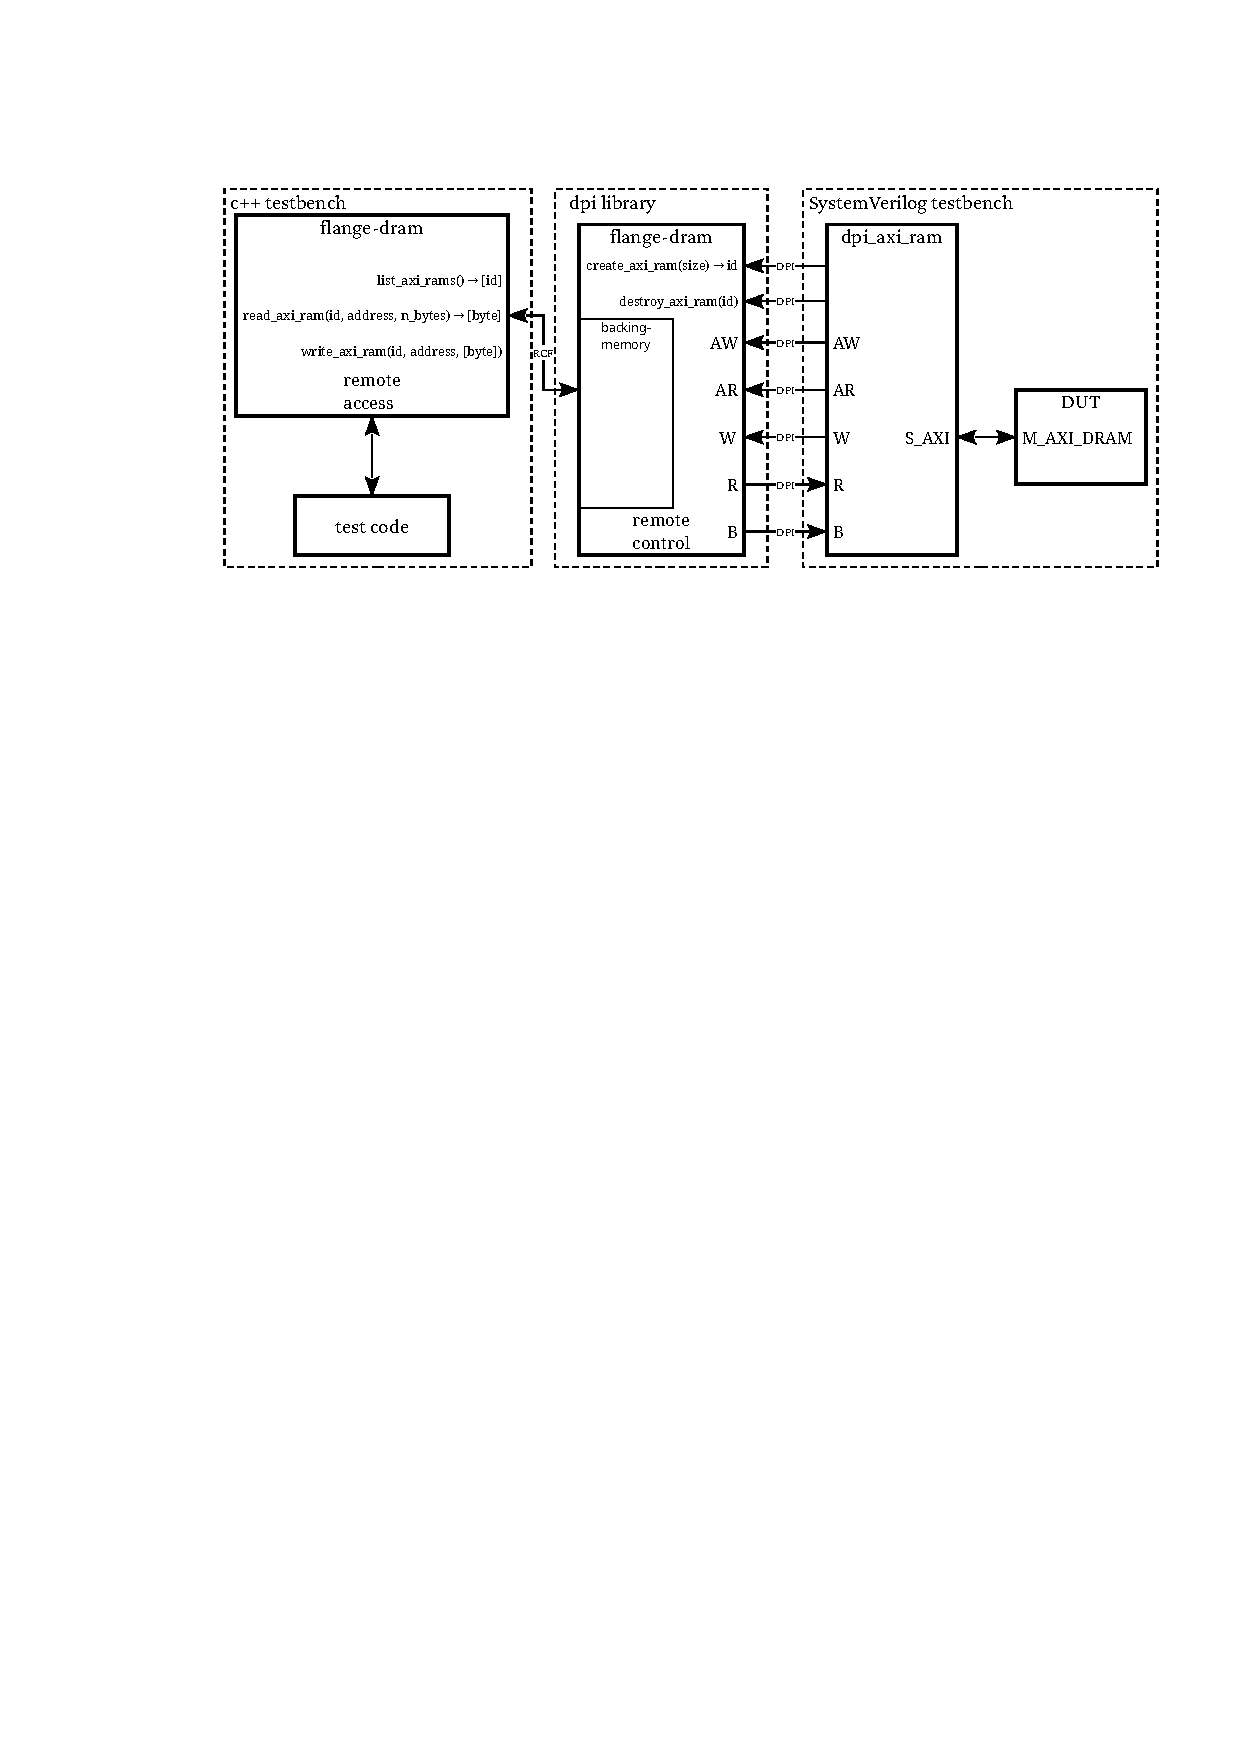
\includegraphics{diagrams/cropped/flange_dram}}
\caption{Schematic overview of \flangedram{} and its interaction with the \cpp{} test suite as well as the \systemverilog{} \DUT{}. \flangedram{} is split into two halves tha communicate via the \RCF{} remote procedure call framework. The first half is a \DPI{} library that exports several functions to be used by the \systemverilog{} code. \code{dpi_axi_ram} is a \systemverilog{} module that has an \AXI{} Subordinate interface and uses the functions exported by the \flangedram{} \DPI{} library to translate the \AXI{} read and write transactions to read and write operations on memory allocated by the \flangedram{} library. This module uses the \code{create_axi_ram} function to create a new memory and receives a \code{id} that identifies this memory. Transactions received on the \AW{}, \AR{} and \W{} \AXI{} channels are communicated to the \DPI{} library, using the \code{id} to identify the memory that they are targeting. Read and write response data is received using the \code{R} and \code{B} functions and converted to transfers on the \R{} and \B{} channels. Every instantiation of the \code{dpi_axi_ram} module creates a separate memory that can have different total sizes of the memory and different \AXI{} data widths.
The second half of \flangedram{} is a library used by the \cpp{} testbench to read and write the contents of the memories created by the \DPI{} library. Using the \code{list_axi_rams} function a list of the \code{id}s corresponding to the memories created by the \DPI{} library can be obtained and the \code{read_axi_ram} and \code{write_axi_ram} are use to read and write from a memory identified by the \code{id}.  }\label{dia:flange-dram-overview}
\end{figure}

\subsubsection{Bandwidth verification}\label{sec:pb_trace_verif}
The new playback and trace generator was designed to be able to sustain the maximum possible bandwidth of the trace and playback streams. However, without verification of this in hardware it is impossible to determine if it is actually able to achieve this bandwidth, due to the limited information on the performance of the \AXIDMA{} and the \XilinxMIG{} given.

For the \AXIDMA{} it is expected it can process the \descriptor{}s at a fixed rate $R$ that is slower than $1$ descriptor per clock cycle. This means that if a sufficiently low buffer length with each \descriptor{} is used the bandwidth of the playback and trace streams will not be limited by the \XilinxMIG{} but instead by this rate $R$.
The minimal buffer length $L$ for which the full playback and trace bandwidth could be reached is then
\[L = \frac{B_{\text{pb\_trace}}}{R}\]
Where $B_{\text{pb\_trace}}$ is the number of bytes that can be transmitted on the playback and trace streams per clock cycle, here $B_{\text{pb\_trace}} = \SI{8}{\byte}$.

To verify the actually achieved bandwidth the \pbexec{} was extended by a dummy data generator. This dummy data generator can be programmed using the \emitDummyInstr{} to emit the programmed number of words on the trace stream. The payload for this dummy data is  an \FPGA{} internal counter that increments with every clock cycle of the \pbexec{} called \systime{}. Dummy words are given the highest priority in the \traceArb{}.
The dummy data generation is mainly used to verify the bandwidth of the trace stream. To verify the bandwidth of the playback stream an instruction that can be processed by the \pbexec{} on every cycle is and has no unwanted side effect is chosen. In this case the \resetSleepInstr{} was used. It resets a counter internal to the \pbexec{} that is not used by the experiments performed here. Finally, every instruction and trace data word used in these experiments has a \UT{} encoding of exactly one \PhyWordSize{} word giving a one to one correspondence between the encoded and the unencoded playback instruction and trace data streams.

The first scenario that is investigated is the maximum bandwidth that can be achieved by the playback stream while minimal trace data is generated while varying buffer length $L$ of the \descriptor{}s used. The \descriptor{} memory has place for $\num{2048}$ \descriptor{}s. One \descriptor{} is needed for the trace data that will contain the value of the \systime{} counter when the first and the last playback instruction was executed, and an additional \descriptor{} is necessary to hold the \haltInstr{} used to mark the end of a \PlaybackProgram{}. This leaves $\num{2046}$ \descriptor{}s that are filled with playback instructions. The first and last playback instruction are \emitDummyInstr{} that each cause the dummy data generator to emit a single dummy word. A single clock cycle is require to execute them and the value of the dummy words is the value of the \systime{} counter when they were generated, which is used to determine value of \systime{} counter when the first and the last playback instruction was executed. All other playback instructions are filled with the \resetSleepInstr{}. The buffer length of each descriptor is varied by varying the number of words $N$ contained in the memory region used by each \descriptor{}. \autoref{fig:pb_benchmark_setup} shows a diagram of the \descriptor{} chains that are generated for this scenario.

As described in \autoref{sec:AXIDMA} the access pattern of a \DDR{} memory can have an influence on the read and write bandwidth that can be achieved. To investigate this effect three different placements of the playback instructions were used:

\begin{enumerate}
    \item With the \linear{} placement all playback instructions are located in the \DDR{} memory in the same order they are executed and therefore read from the memory.
    \item With the \random{} placement the location of each region of memory used for each \descriptor{} is randomized.
    \item With the \randomDense{} placement the location of each region of memory used for each \descriptor{} is randomized, but no gaps are allowed.
\end{enumerate}

\begin{figure}[htbp]
\centerline{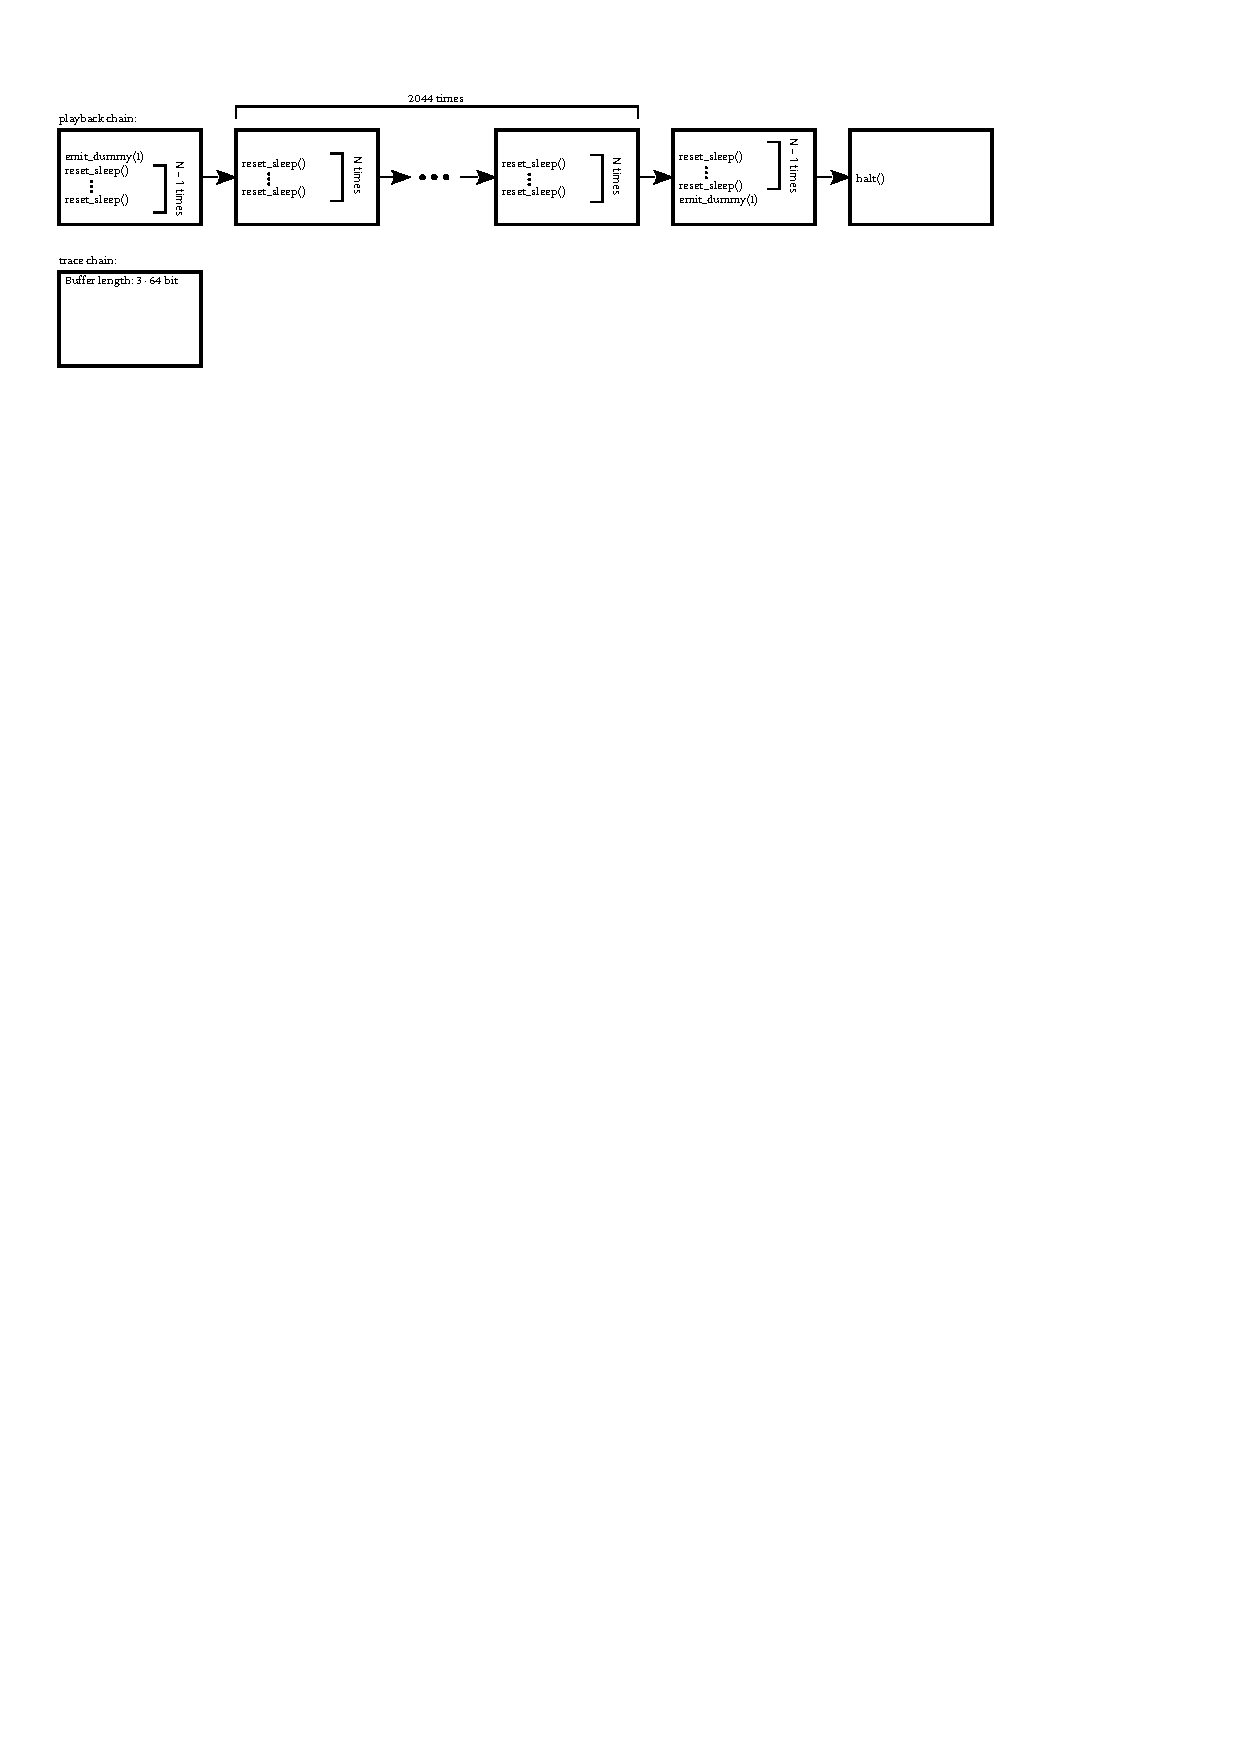
\includegraphics{diagrams/cropped/benchmark_pb}}
\caption{Schematic overview of the playback and trace buffer chains used to measure the playback bandwidth.}\label{fig:pb_benchmark_setup}
\end{figure}

The second scenario investigates the maximum bandwidth that can be achieved by the trace stream while minimal words are transmitted on the playback stream. A single \descriptor{} is used for the playback stream, that first configures a long timeout to avoid interruption of the generation of the dummy trace data by a timeout notification. It configures the dummy data generator to generate dummy trace data and after waiting for the dummy data generator to be idle terminates the \PlaybackProgram{} using the \haltInstr{}. The looped back \haltInstr{} is received by its own trace \descriptor{}. The other $\num{2046}$ trace descriptors are configured in one single \descriptor{} chain. The number of words $N$ that is received by each \descriptor{} is varied. Finally, for the placement of the trace memory region used by each of the \descriptor{} the same three placement strategies as for the first scenario are used. In this case the number of clock cycles that were needed to receive the whole trace data can be determined by comparing the \systime{} value of the first and the last dummy word that is written to the trace memory. \autoref{fig:trace_benchmark_setup} shows an overview of the \descriptor{} chains used in this scenario.

\begin{figure}[htbp]
\centerline{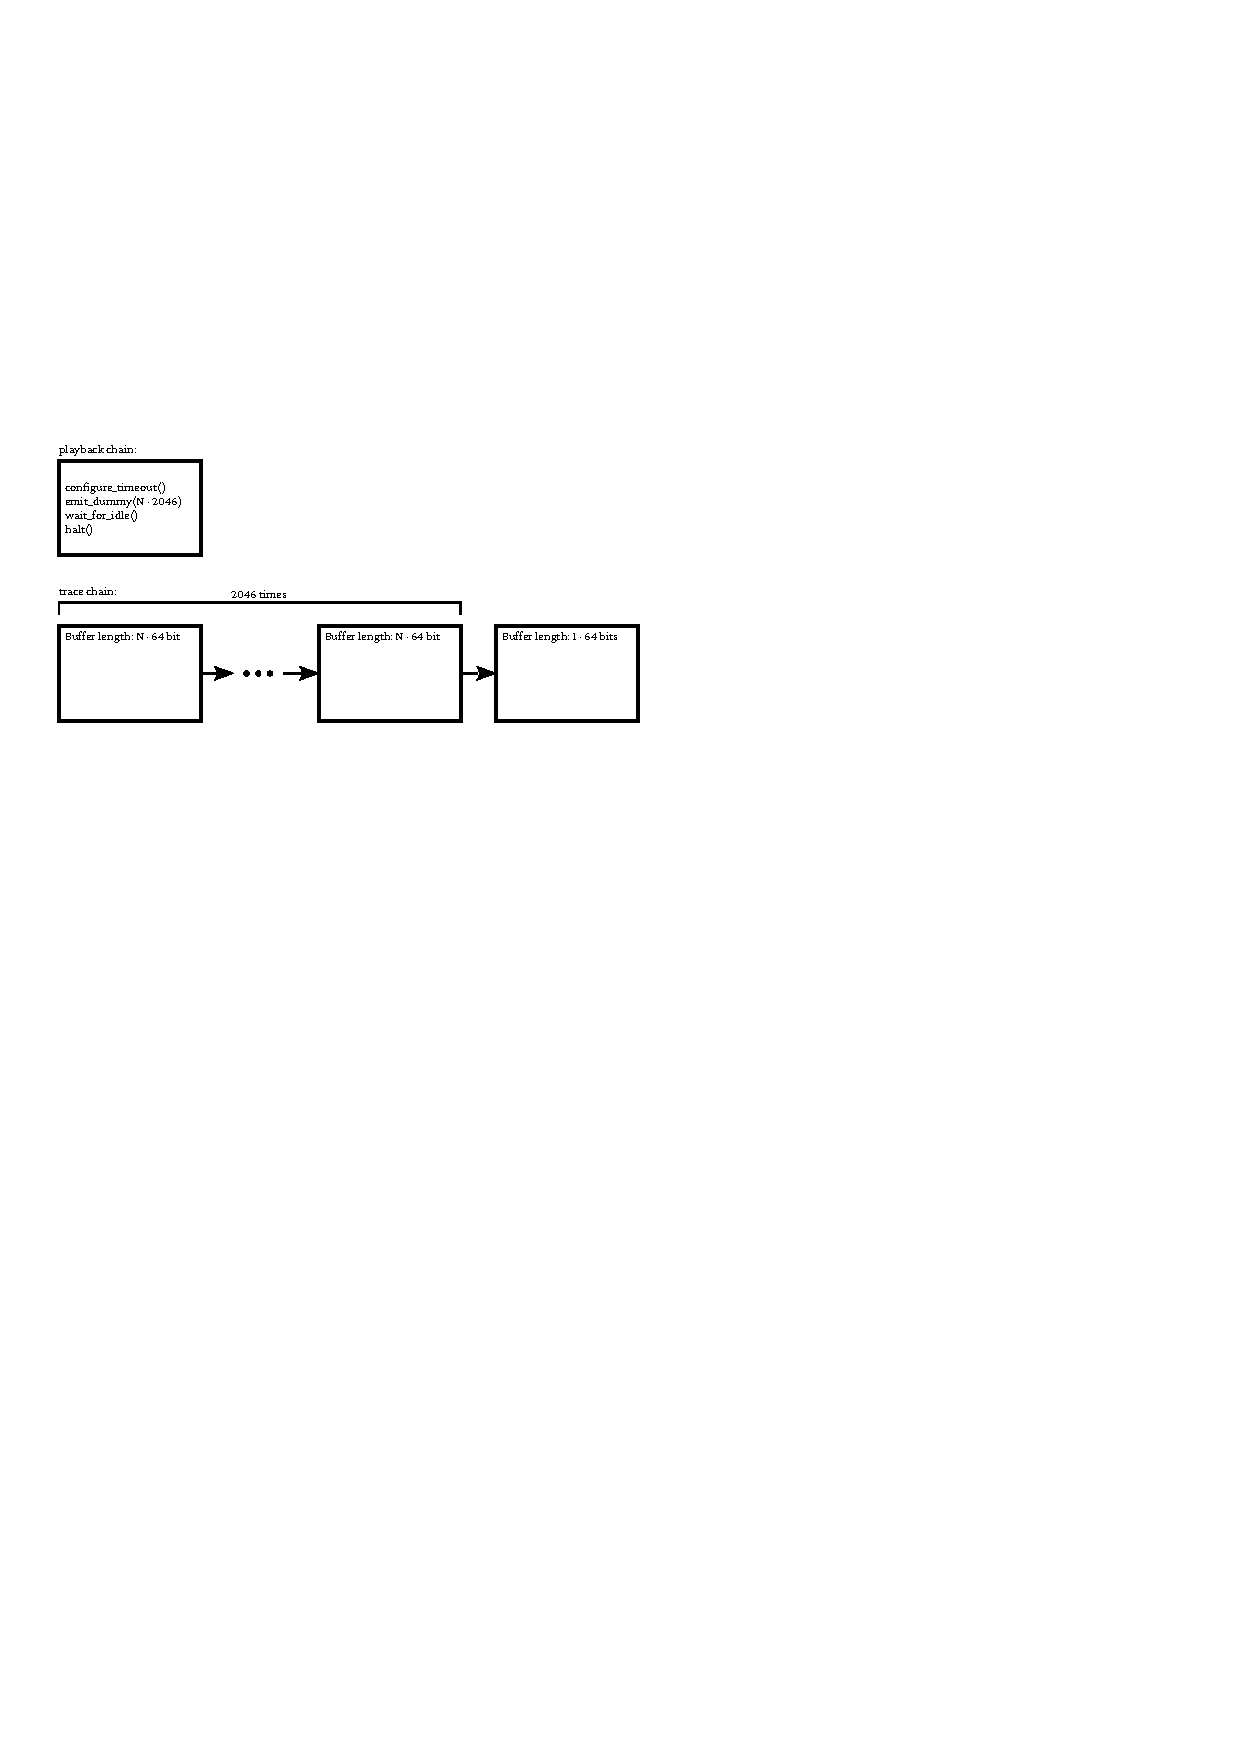
\includegraphics{diagrams/cropped/benchmark_trace}}
\caption{Schematic overview of the playback and trace buffer chains used to measure the trace bandwidth}\label{fig:trace_benchmark_setup}
\end{figure}

At last the third scenario measures the maximum bandwidth achieved on the playback and trace streams when both are used at the same time. Using the dummy data generator the \pbexec{} is configured to generate the same number of trace words as it will receive playback instructions. One playback \descriptor{} is used in the beginning to configure the timeout already mention in the second scenario. Furthermore, an additional \descriptor{} is used for the playback chain that contains the \haltInstr{} used to indicate the end of a \PlaybackProgram{}, which is looped back to a third \descriptor{} used in the trace chain. The remaining $\num{2045}$ are split evenly between the playback and the trace chain. One \descriptor{} stays unused. The first instruction in the playback stream after the timeout configuration configures the dummy data generator to emit the number of dummy words necessary to fill the trace \descriptor{} chain, while the last instruction before the \haltInstr{} causes \systime{} counter to be read from  an \FPGA{} internal bus. This will cause the value of the \systime{} counter one clock cycle after it was executed to be placed into a \FIFO{} internal to the \pbexec{} where it will remain until it can be written to the trace stream. As the dummy data generator has the highest priority this can only happen after all dummy data was generated and therefore does not influence the trace stream. \autoref{fig:pb_trace_benchmar_setup} gives an overview of the playback and trace chains that are generated for this case.

In this case again the number of words $N$ used in each \descriptor{} and the placement of the playback instructions and the trace data varied.
Here five different configurations for the placement were investigated:
\begin{enumerate}
  \item \linear{} placement, that places all playback instructions is the same order as they are executed, and also places the trace data for each \descriptor{} consecutively.
  \item \random{} placement that randomizes the location of each region of playback instructions and trace data
  \item \randomDense{} placement that randomizes the location of each region of playback instructions and trace data while not leaving any gaps
  \item \interleaved{} placement that places the playback instructions and the trace data into alternating regions leaving gaps between each of them
  \item \interleavedDense{} placement that places the playback instructions and the trace data into alternating consecutive regions
\end{enumerate}

\begin{figure}[htbp]
\centerline{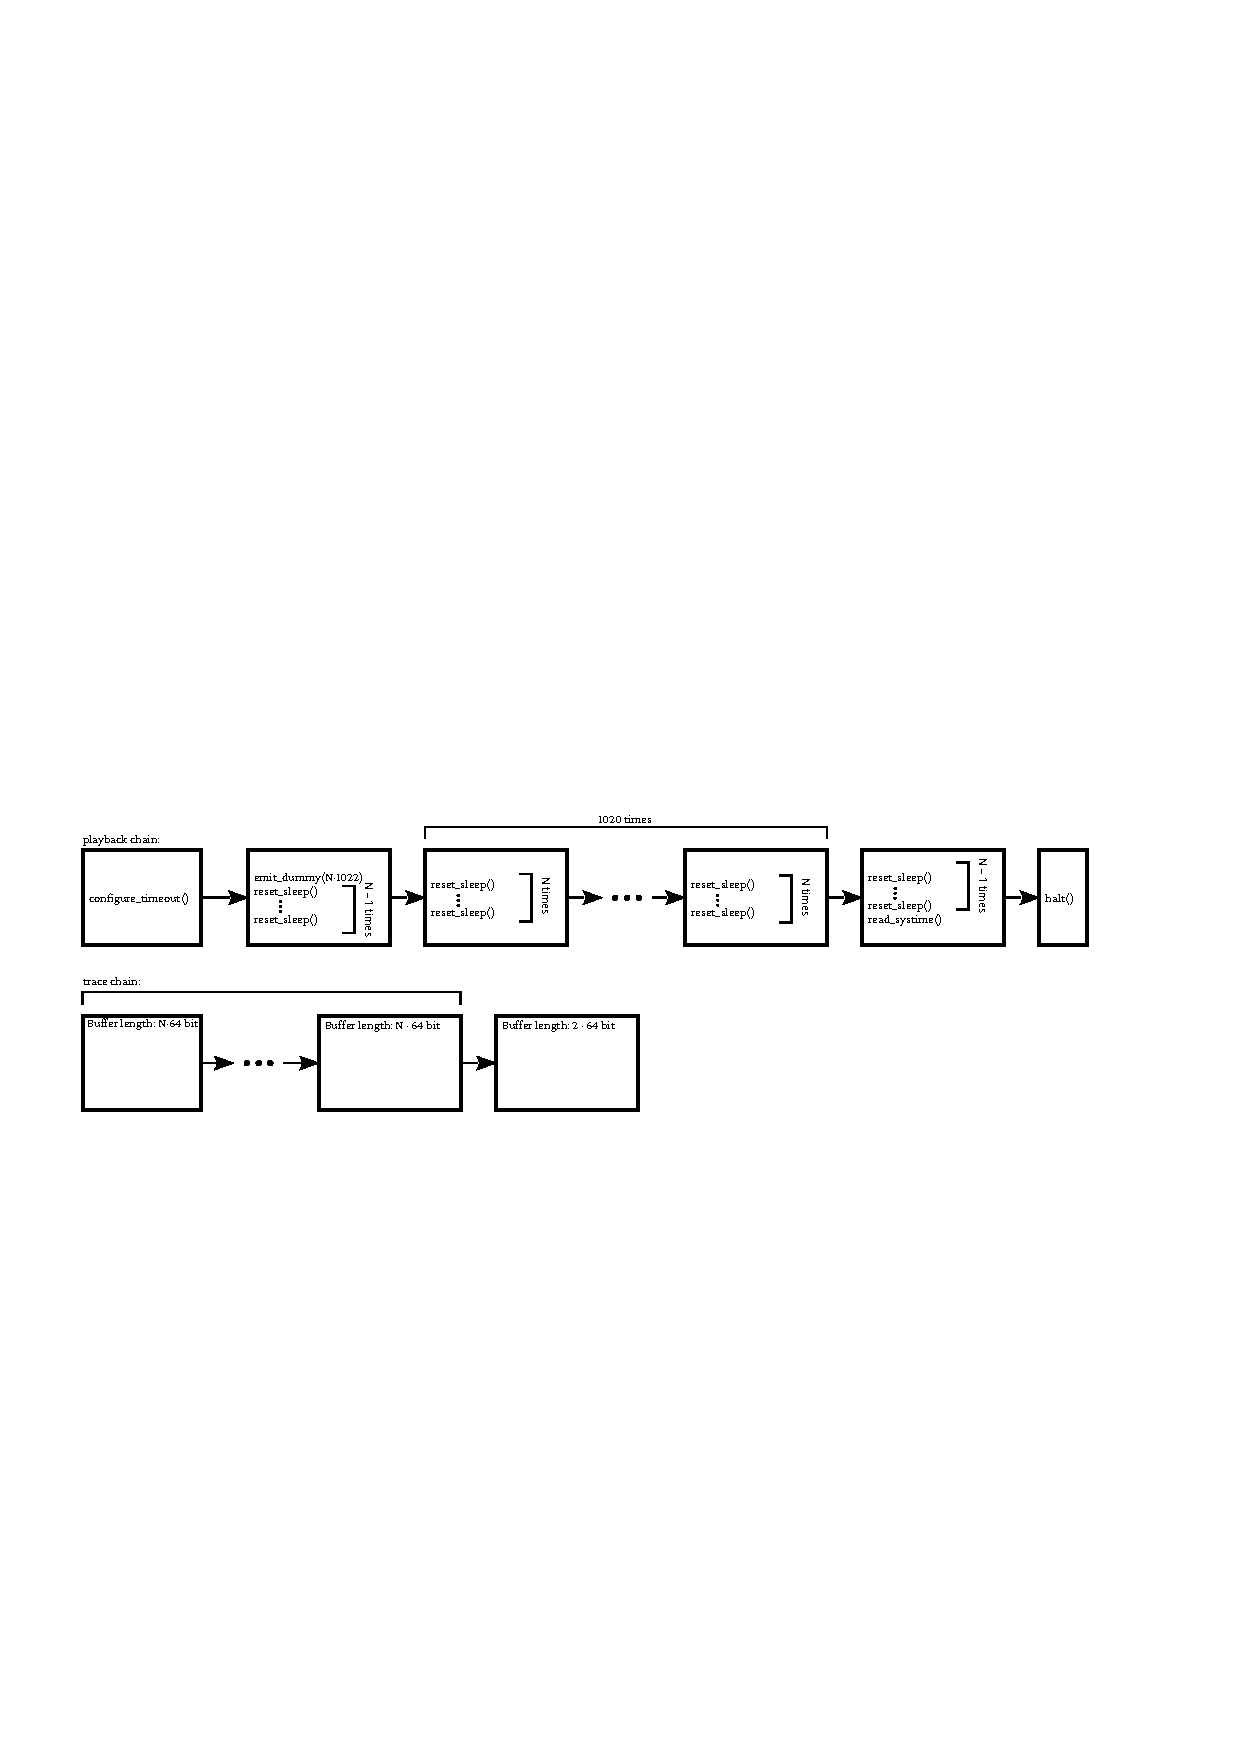
\includegraphics{diagrams/cropped/benchmark_pb_trace}}
\caption{Schematic overview of the playback and trace buffer chains used to measure simultaneous playback and trace bandwidth}\label{fig:pb_trace_benchmar_setup}
\end{figure}

\section{Results}
\subsection{Playback and trace bandwidth}\label{sec:pb_trace_bw}
The playback and trace bandwidth is measured for the tree scenarios that were described in \autoref{sec:pb_trace_verif}. For the four different choices for the design of new playback and trace management block were are compared. The following highlights the downsides of the $\PhyWordSize{}$ option for the $W$ parameter and the advantage of the \texttt{playback} as well as the \texttt{trace FIFO}.

\autoref{fig:pb_128_no_fifo} shows the playback bandwidth for $W = \SI{128}{\bit}$ and no \texttt{playback FIFO}. As expected for small buffer lengths the maximum bandwidth cannot be achieved. \autoref{fig:pb_128_no_fifo_zoom} shows the experiment with the limits of the \(y\)-axis adjusted to show only a small region around the maximum possible bandwidth. This shows that for some buffer lengths the playback stream is not always able to achieve the maximum possible bandwidth. In fact there is no buffer length where the minimum achieved bandwidth was always equal to the maximum one.
\begin{figure}[!htbp]
\inputpgf{data/pb_bandwidth_128_no_fifo.pgf}\label{fig:pb_128_no_fifo}
\caption{Measured bandwidth of the playback stream for $W = \SI{128}{\bit}$ and no \texttt{playback FIFO} for the three memory placements. Each tested buffer length was repeated $\num{1000}$ times and the minimum bandwidth is shown.}
\end{figure}

\begin{figure}[!htbp]
\inputpgf{data/pb_bandwidth_128_no_fifo_zoom.pgf}\label{fig:pb_128_no_fifo}
\caption{Measured bandwidth of the playback stream for $W = \SI{128}{\bit}$ and no \texttt{playback FIFO} for the \random{} memory placements. Each tested buffer length was repeated $\num{1000}$ times the distribution of the measured bandwidths is visualized using a violin plot. The horizontal bars indicate the minimum and maximum measured bandwidth. The \(y\)-axis is limited to a small region around the maximum bandwidth.}
\end{figure}


\autoref{fig:pb_128_fifo} shows the playback bandwidth for $W = \SI{128}{\bit}$ and using the \texttt{playback FIFO}. Again as expected for small buffer lengths the maximum bandwidth cannot be achieved. \autoref{fig:pb_128_fifo_zoom} shows the same zoomed in region as \autoref{fig:pb_128_no_fifo}. In contrast to the version without the \texttt{playback fifo} the bandwidth of the playback stream is never below the maximum bandwidth for any buffer length greater than or equal to $\num{\PBMinBSForlinear} · \PhyWordSize{}$.

\begin{figure}[!htbp]
\inputpgf{data/pb_bandwidth_128_fifo.pgf}\label{fig:pb_128_fifo}
\caption{Measured bandwidth of the playback stream for $W = \SI{128}{\bit}$ and using the \texttt{playback FIFO} for the three memory placements. Each tested buffer length was repeated $\num{1000}$ times and the minimum bandwidth is shown.}
\end{figure}

\begin{figure}[!htbp]
\inputpgf{data/pb_bandwidth_128_fifo_zoom.pgf}\label{fig:pb_128_fifo_zoom}
\caption{Measured bandwidth of the playback stream for $W = \SI{128}{\bit}$ using the \texttt{playback FIFO} for the \random{} memory placements. Each tested buffer length was repeated $\num{1000}$ times and the minimum bandwidth is shown. The \(y\)-axis is limited to a small region around the maximum bandwidth.}
\end{figure}


\autoref{fig:trace_128_fifo} shows the measured trace bandwidth for $W = \SI{128}{\bit}$ and no \texttt{trace FIFO}. As expected and similar to the playback stream, the maximum bandwidth is not reached for small buffer lengths. For any buffer length greater than or equal to $\num{\PBMinBSForlinear}$ the minimum bandwidth measured matches the maximum possible bandwidth.
\begin{figure}[!htbp]
\inputpgf{data/trace_bandwidth_128.pgf}\label{fig:trace_128_fifo}
\caption{Measured bandwidth of the trace stream for $W = \SI{128}{\bit}$ and no \texttt{trace FIFO}. Each tested buffer length was repeated $\num{1000}$ times and the minimum bandwidth measured is shown.}
\end{figure}


% pb linear 64.0
% trace linear 16384.0
% pb random 64.0
% trace random 2048.0
% pb random_dense 68.0
% trace random_dense 16384.0
% pb interleaved 64.0
% pb interleaved_dense 64.0

\autoref{fig:pb_trace_64} shows the measured trace and playback bandwidths for $W = \SI{64}{\bit}$. While the playback stream is able to reach the maximum possible bandwidth for every buffer length greater than or equal to $\num{68} · \PhyWordSize$, the trace stream cannot reach the maximum bandwidth for every of the memory placement patterns. Indeed only the \linear{}, \random{} and the \randomDense{} memory placement patterns are able to achieve the maximum possible bandwidth, however they only reach it for a buffer length greater than or equal to $\num{16384} · \PhyWordSize$, $\num{2048} · \PhyWordSize$ and $\num{16384} · \PhyWordSize$ respectively.

\begin{figure}[!htbp]
\inputpgf{data/pb_trace_bandwidth_64.pgf}\label{fig:pb_trace_64}
\caption{Measured bandwidth of the playback and trace stream for $W = \SI{64}{\bit}$. Each tested buffer length was repeated $\num{1000}$ times and the minimum bandwidth measured is shown. The color of the points encodes the memory placement pattern that was used.}
\end{figure}

\autoref{fig:pb_trace_128} shows the measured trace and playback bandwidths using the \texttt{playback FIFO} but without the \texttt{trace FIFO} for $W = \SI{128}{\bit}$. The playback stream is able to reach the maximum possible bandwidth for every buffer length greater than or equal to $\num{68} · \PhyWordSize$, and in contrast to the $W = \SI{64}{\bit}$ the trace stream can reach the maximum bandwidth for every of the memory placement patterns. However it is only reached for all memory access pattern for buffer lengths greater than or equal to $\num{720} · \PhyWordSize$.
\begin{figure}[!htbp]
\inputpgf{data/pb_trace_bandwidth_128_fifo.pgf}\label{fig:pb_trace_128}
\caption{Measured bandwidth of the playback and trace stream for $W = \SI{128}{\bit}$ with the \texttt{playback FIFO} and without the \texttt{trace FIFO}. Each tested buffer length was repeated $\num{1000}$ times and the minimum bandwidth measured is shown. The color of the points encodes the memory placement pattern that was used.}
\end{figure}

Finally \autoref{fig:pb_trace_128_both_fifo} shows the measured trace and playback bandwidths using the \texttt{playback FIFO} together with the \texttt{trace FIFO} for $W = \SI{128}{\bit}$. As without the \texttt{trace FIFO} the playback stream is able to reach the maximum bandwidth for any buffer length greater than or equal to $\num{68} · \PhyWordSize$ however the minimum buffer length required to reach the maximum bandwidth on the trace stream is reduced to $80 · \PhyWordSize$.

\begin{figure}[!htbp]
\inputpgf{data/pb_trace_bandwidth_128_both_fifo.pgf}\label{fig:pb_trace_128_both_fifo}
\caption{rate}
\caption{Measured bandwidth of the playback and trace stream for $W = \SI{128}{\bit}$ with both the \texttt{playback} and the \texttt{trace FIFO}. Each tested buffer length was repeated $\num{1000}$ times and the minimum bandwidth measured is shown. The color of the points encodes the memory placement pattern that was used.}
\end{figure}

For the following experiments only the version with $W = \SI{128}{\bit}$ and both the \texttt{playback} and the \texttt{trace FIFO} will be used.

\autoref{fig:pb_vs_stock}, \autoref{fig:trace_vs_stock} and \autoref{fig:pb_trace_vs_stock} show comparisons between the playback, trace and simultaneous playback and trace bandwidth depending on the size of the \PlaybackProgram{} and or generated trace data. These bandwidths are measured using a modification of the tests described in \autoref{sec:pb_trace_verif}. Instead of using the maximum number of \descriptor{}s possible the minimum number of \descriptor{}s that are needed to hold the complete \PlaybackProgram{} trace data is used.

The new playback and trace management achieves the maximum bandwidth regardless of the size of the \PlaybackProgram{} and or generated trace data. In contrast to that the old playback and trace management is not able to achieve the maximum bandwidth. This is expected for very large trace data and \PlaybackProgram{}s, as it is only able to store $\SI{32}{\mebi\byte}$ of trace data and \PlaybackProgram{} instructions. \PlaybackProgram{}s greater than $\SI{32}{\mebi\byte}$ are limited by the bandwidth between the host and the \FPGA{} as the instructions for them will be transmitted during their execution. The same applies to trace data bigger than $\SI{32}{\mebi\byte}$, which is only accepted from the \pbexec{} at the rate it can be sent to the host.
In addition to that these measurements also reveal that the old playback and trace management is not able to achieve the full playback and trace bandwidth for \PlaybackProgram{}s and or trace data smaller than $\SI{32}{\mebi\byte}$.
\begin{figure}
\inputpgf{data/pb_new_vs_stock_bandwidth.pgf}\label{fig:pb_vs_stock}
\caption{Measured playback bandwidth of the old and the new playback management. For each size of the \PlaybackProgram{} the bandwidth was measured $\num{100}$ and visualized using a violin plot. The three horizontal bars indicate the minimum, average and maximum measured bandwidth.}
\end{figure}

\begin{figure}
\inputpgf{data/trace_new_vs_stock_bandwidth.pgf}\label{fig:trace_vs_stock}
\caption{Measured playback bandwidth of the old and the new playback management. For each size of the \PlaybackProgram{} the bandwidth was measured $\num{100}$ and visualized using a violin plot. The three horizontal bars indicate the minimum, average and maximum measured bandwidth.}
\end{figure}

\begin{figure}
\inputpgf{data/pb_trace_new_vs_stock_bandwidth.pgf}\label{fig:pb_trace_vs_stock}
\caption{Measured playback bandwidth of the old and the new playback management. For each size of the \PlaybackProgram{} the bandwidth was measured $\num{100}$ and visualized using a violin plot. The three horizontal bars indicate the minimum, average and maximum measured bandwidth.}
\end{figure}

\subsection{\FAXI{} based memory mapped communication}
The \rtt{} and the bandwidth of the \FAXI{} based \AXI{} master over \HostARQ{} is measured. All measurements were performed from the same host computer (\testnode{}) reserved exclusively for these tests.
To measure the \rtt{} minimum size reads and write of $\SI{8}{\byte}$ from multiple \AXI{} slaves is performed. For reads the time elapsed between the transmission of the header and address and the reception of the read data is measured, while for writes the time elapsed between the transmission of the write transaction and the reception of the write response is measured. The measured \rtt{} can is visualized in \autoref{fig:faxi-rtt} and table \autoref{tbl:rtt} summarizes the average latency that was measured.

\begin{table}
  \begin{center}
\begin{tabular}{lll}
  \toprule
  action & location & \rtt{} \\
  \midrule
  read & \DDR{} memory & \MeanStdValue{FAXIRTTReadDDR}{\nano\second} \\
  write & \DDR{} memory & \MeanStdValue{FAXIRTTWriteDDR}{\nano\second} \\
  read & \AXIDMA{} register & \MeanStdValue{FAXIRTTReadAXI}{\nano\second} \\
  write & \AXIDMA{} register & \MeanStdValue{FAXIRTTWriteAXI}{\nano\second} \\
  read & \descriptor{} memory & \MeanStdValue{FAXIRTTReadSG}{\nano\second} \\
  write & \descriptor{} memory & \MeanStdValue{FAXIRTTWriteSG}{\nano\second} \\
  \bottomrule
\end{tabular}
  \end{center}
\caption{Summary of the \rtt{} measured for read and write operations from to different \AXI{} slaves}\label{tbl:rtt}
\end{table}

\begin{figure}
\inputpgf{data/faxi_rtt.pgf}\label{fig:faxi-rtt}
\caption{\rtt{} of reads and writes of $\SI{8}{\byte}$ from multiple different \AXI{} slaves. Each operation was performed $\num{10000}$ times and a is summarized using a violin plot. The three bars show the mean as well as the first and $99$th percentile}
\end{figure}

The bandwidth for reads and write to the \DDR{} memory was measured for different read and write sizes, by measuring the time that elapses between sending of the read and write transactions and the reception of their response. A baseline maximum bandwidth for sending to the \FPGA{} and for data sent from the \FPGA{} of the \HostARQ{} protocol was measured by sending \HostARQ{} traffic to a test sink built into the \FPGA{} implementation of the \HostARQ{} protocol as well as by using a dummy data generator built into the design as well. For sending data to the \FPGA{} a baseline bandwidth of \MeanStdValue{hostarqWriteBw}{\byte\per\second} was measured and for reception of data from the \FPGA{} a baseline bandwidth of \MeanStdValue{hostarqReadBw}{\byte\per\second}. \autoref{fig:faxi_read_bw} shows the read bandwidth that was measured and \autoref{fig:faxi_write_bw} the write bandwidth.

\begin{figure}
\inputpgf{data/faxi_read_bw.pgf}
\caption{Read bandwidth for reads from the \DDR{} memory of different sizes using \FAXI{}. For each size the bandwidth was measured $\num{100}$ times and is summarized using a violin plot. The three bars show the mean as well as the first and $99$th percentile. The horizontal line is the limit for \HostARQ{} measured previously.}\label{fig:faxi_read_bw}
\end{figure}

\begin{figure}
\inputpgf{data/faxi_write_bw.pgf}
\caption{Write bandwidth for writes from the \DDR{} memory of different sizes using \FAXI{}. For each size the bandwidth was measured $\num{100}$ times and is summarized using a violin plot. The three bars show the mean as well as the first and $99$th percentile. The horizontal line is the limit for \HostARQ{} measured previously.}\label{fig:faxi_write_bw}
\end{figure}

\subsection{Experiment rate}
Finally the rate of experiments that can be performed in a \HWinTheLoop{} fashion is measured. The experiment that was used to test this is the same one used to determine the simultaneous playback and trace stream bandwidth and the size of the \PlaybackProgram{} and the generated trace data is varied. \autoref{fig:experimentrate} shows a comparison between the experiment rate that is achieved using the playback and trace management presented in this thesis and the old playback and trace management. To determine the rate, the duration of the execution of a single experiment including the creating of the \PlaybackProgram{} and the reception of the trace data is measured. As can be seen in \autoref{fig:experimentrate} as expected for very small \PlaybackProgram{}s the \rtt{} dominates the time required to perform an experiment and the new playback and trace management is at least two times slower than old playback and trace management (because it needs at least two round trips to perform a single experiment). Furthermore the experiment rate of the new trace and playback management is always lower than the old one as the trace data is only read out once experiment is completed. Before that it not know how much trace data was actually generated and written to the \DDR{} memory by the \AXIDMA{}. The old trace and playback management can send the trace data as it is generated. As the experiment rate is mainly limited by the bandwidth of the connection between the host and the \FPGA{} the effect of these differences deceases with increasing playback and trace size until the rate for the new and the old is very close.
Finally the measurements show that the ratio between the rate of experiments with the old and the new playback management increases again for the old trace and playback management for \PlaybackProgram{}s that are larger than $\SI{32}{\mebi\byte}$. This is caused by the playback memory in the old playback and trace management being filled up for \PlaybackProgram{}s that are larger than $\SI{32}{\mebi\byte}$ which causes the execution of the \PlaybackProgram{} to be started before it is received completely and the transmission of the playback program from the host and the execution overlap. The new playback and trace management can use the whole size of the \DDR{} memory and the execution of the \PlaybackProgram{} is not started until it is received completely.
\begin{figure}
\inputpgf{data/experiment_rate.pgf}
\caption{Comparison of the rate of experiments between the old and the new playback and trace management. For each size the time required to perform a single experiment was measured $\num{100}$ times. In green the ration between the experiment rate of the old and the new playback and trace management is shown. The vertical line indicates the location of $\SI{32}{\mebi\byte}$ on the $x$-axis}\label{fig:experimentrate}
\end{figure}

\subsection{flange-dram performance}
\autoref{fig:flange_perf} shows a comparison between the time that is required to perform a test case part of the \hxcomm{} test suite that reads the \JTAGID{} of the \ASIC{} when using the simulation backend of \hxcomm{} depending on the \AXI{} \DDR{} simulation model used. For this test \xcelium{} with version \xceliumVer{} was used. The test case is performed $\num{10}$ times in sequence and each repetition is shown separately. One can see that the \XilinxMIG{} and \DDR{} based simulation is a lot slower than the other two options. Furthermore the first repetition of the test case requires almost double the time of all following repetitions, when using the \XilinxMIG{} based simulation. This is caused by the link training that is performed before the \XilinxMIG{} can operate. The other two simulation models do not require this link training phase. On average one execution of the test case requires \MeanStdValue{DramAll}{\second} for the \XilinxMIG{} and \DDR{} simulation model option, \MeanStdValue{FlangeDram}{\second} when using \flangedram{} and \MeanStdValue{SimBram}{\second} when using the simulation model using block ram.


\begin{figure}
\inputpgf{data/flange_dram_perf.pgf}
\caption{Number of seconds required by the \hxcomm{} test case that reads the \JTAGID{} of the \ASIC{} using a \FPGA{} and \ASIC{} simulation as target. The three different choices for the \AXI{} \DDR{} memory simulation model evaluated, the \XilinxMIG{} in combination with a \DDR{} simulation model, \flangedram{} and the block ram based option. The \hxcomm{} test case is repeated $\num{10}$ times in series and the time required for each shown separately. Each point is measured 10 times.}\label{fig:flange_perf}
\end{figure}

\subsection{\FPGA{} resources usage}


\todo{maybe playback and trace bw while reading the trace? (pb rate drops :(, we need priority in the interconnect)}

\section{Summary and discussion}
This thesis aimed to provide a new design for the playback and trace buffer that improves the old design on multiple fronts
\begin{itemize}
\item Usage of the complete $\DDRSIZE{}$ of storage available
\item The ability to reuse (parts of) already transmitted \PlaybackProgram{}s
\item The ability to read back the trace data in a different order than it was generated.
\item Deterministic timing for the execution of any \PlaybackProgram{}s split into blocks of atleast $\num{68} · \PhyWordSize{}$.
\end{itemize}
To achieve these goals the operation of the playback and trace buffer was redesigned from the ground. An \FPGA{} module that allows memory mapped access from the host and uses a scatter gather \DMA{} engine to construct the stream of playback instructions from multiple (potentially out of order) blocks was developed. Integration with the \BSSTwo{} software stack was performed. A new software layer called \ayo{} that is responsible for the low level interaction with the playback and trace buffer parts, such as reads and writes to the \DDR{} memory holding the playback and trace data aswell as the configuration of the \DMA{} engine was implemented. \ayo{} exposes an interface that allows usage of the new functionality, like the reuse of parts of the \PlaybackProgram{}s and partial readout of the trace data. Basic integration of \ayo{} with the \hxcomm{} layer was performed, that allows all current software to use the new playback and trace buffer design without any modifications, gaining the ability to use the much bigger $\DDRSIZE{}$ of storage available.

This new design for the playback buffer and software integration was tested extensively and compared in detail to the old design. For these tests and comparisons, the simulation environment was extended by a software accessible \AXI{} \DRAM{} and the \FPGA{} design was extended by a dummy data generator used to generate arbitrary amounts of trace data at maximum data rate.

It was verified that the software layer and memory mapped access to the \DDR{} memory is able to achieve a similar bandwidth between the host and the \FPGA{} as the old way of communication with the \FPGA{}.

The only disadvantage of the new playback and trace buffer is the reduced rate of experiments that can be performed in a \HWinTheLoop{} fashion.
For \PlaybackProgram{}s with a size of at least $\SI{1392}{\byte}$ and a trace data size of at least$\SI{1392}{\byte}$ the rate experiments that is possible with the new playback and trace buffer design was show to be less than two times lower than the rate for the old design. For any size of \PlaybackProgram{} and generated trace data, the rate of experiments was always less than $5$ times lower. The lower rate of experiments is caused by
additional \rtt{}s that are necessary between the \FPGA{} and the host and \autoref{sec:latency_reduction} outlines options for further extensions of this playback and trace buffer design to reduce the number of \rtt{}s required and therefore increase the rate of experiments again.
It was demonstrated that the complete size of the \DDR{} memory is possible to be used instead of only $\SI{64}{\mebi\byte}$ used by the old buffer design.

Finally, it was verified that for \PlaybackProgram{} constructed from blocks of at least $\num{68}·\PhyWordSize{}$ and for trace data organized into blocks of at least $\num{80}·\PhyWordSize{}$, the new playback and trace buffer always achieves the maximum possible bandwidth. This was verified to hold even for a variety of possible placements of these blocks in the \DDR{} memory space.
This constitutes a mayor improvement over the old playback and trace buffer design, which is not able to sustain this the maximum possible bandwidth for many \PlaybackProgram{} and or trace sizes and drastically improves the reliablity.

\section{Outlook}\label{sec:outlook}
The new memory mapped playback and trace buffer and the software integration presented in this thesis lays a foundation for a lot of future improvements of the \BSS{} stack.
\subsection{Latency reduction}\label{sec:latency_reduction}
The only disadvantage of the new playback and trace buffer is that for small \PlaybackProgram{}s the rate of experiments that can be performed in a \HWinTheLoop{} fashion is significantly lower than the rate of experiments that can be performed with the old design. This could be improved using one of several approaches
\subsection{Higher level software integration}
The \ayo{} software layer already exposes the new functionality of the new playback and trace buffer such as the ability to reuse block of already transmitted \PlaybackProgram{}s and partial readout of the generated trace data. However, this is functionality is not yet used by the upper layer of the \BSS{} software stack. As the rate with which experiments that can be performed is limited by the bandwidth between the host and the \FPGA{} for \PlaybackProgram{}s or trace data greater than $\SI{1392}{\byte}$, integration of this functionality with higher level software is expected to allow the rate of some experiments to be improved.
\begin{itemize}
  \item The \AXIDMA{} provides an interrupt signal that is asserted whenever the processing of a \descriptor{} is completed. These interrupts could be used to avoid the need for polling of the trace descriptor status.
  \item Introduction of a separate low latency path for the trace data, that bypasses the playback and trace buffer and instead is sent directly to the host, similar to the old trace buffer.
  \item Introduction of memory mapped access from the \FPGA{} to the host, to allow the \FPGA{} to write the host memory directly. This could for example be achieved by implementation of a module similar to \FAXI{} but operating is an opposite direction and providing an \AXI{} Subordinate interface to the \FPGA{}.
\end{itemize}
\subsection{Unified memory with PPU}
The \BSSTwo{} architecture includes microcontrollers on the \ASIC{} that allow for sophisticated on chip processing. They can for example be used for closed loop operation of the \ASIC{}. The \FPGA{} is connected to a \DDR{} memory, independent from the \DDR{} memory used for the playback and trace buffer, that provides working memory for these microcontrollers, that is used additionally to the on-chip \SRAM{}. In the futures it is envisioned to allow memory mapped access to this \DDR{} by the host using \FAXI{} and furthermore, the microcontrollers are envisioned to access the playback and trace memory, descriptor memory and \AXIDMA{} register space as well, to allow configuration directly from the microcontroller.
\subsection{Support of new host interfaces}
The old playback and trace buffer was tightly coupled to the stream interface of the \HostARQ{} protocol. By replacing the \FAXI{} module, the new playback and trace buffer design can be used with any host interface as long as one provides a bridge between the host interface and the \AXI{} bus. Using this one could for example use \PCIe{} instead of \UDP{} as the communication interface between the \FPGA{} and the host.

% \section{Outlook}
\subsection{Full Stack scatter gather integration}
\subsection{AXIDMA interrupt integration}
\subsection{low latency trace data}
\subsection{unified memory with PPU}


\printbibliography
\section*{Erkl\"{a}rung}

Ich versichere, dass ich diese Arbeit selbstst\"{a}ndig verfasst und keine anderen als die angegebenen Quellen und Hilfsmittel benutzt habe.

Heidelberg, den ...,

%Unterschrift


\end{document}
